\colorlet{proofmatt}{white}


On one hand, PDGs are powerful modeling tools, and representations of uncertainty.
On the other, PDGs are universal loss functions. 
This chapter describes a deep connection between two roles of PDGs. 
We start with a suggestive observation: that the semantics by which PDGs specify a distribution is equivalent to the semantics that simply evaluates a PDG's degree of inconsistency (\cref{sec:semantic-connection}). 
We then build on this semantic connection by describing a surprisingly strong algorithmic one: an inconsistency oracle can be used to perform inference (\cref{sec:deeper-connection-overview}) in almost-linear time. 
% To do this precisely, we must also formally describe the problems of approximate inference and inconsistency (\cref{sec:approximate-inference}).
% We prove  (rather substantial) proof to \cref{proofs:the-reductions}.
% In this sense, precisely quantifying one's inconsistencies is no easier than optimally resolving them.  
Thus, the two views of PDGs are essentially equivalent---not only semantically, but algorithmically as well.

In between, we formally describe the two computational problems of interest in \cref{sec:approximate-inference}, and finish off the upper bounds developped in \cref{chap:infer}.

 
% \section{A Semantic Connection}
\section{A Semantic Connection}
    \label{sec:semantic-connection}

% Recall that the inconsistency of a PDG is the score of its best-scoring distribution:
% \[
%     \aar{\dg M}_\gamma := \inf_{\mu \in \Delta \V\!\X} \bbr{\dg M}_\gamma(\mu).
% \]
Recall that we defined the inconsistency $\aar{ \,\cdot\, }$ of a PDG is the score of its best-scoring distribution.
Although we defined
$\aar{ \,\cdot\, }$
in terms of the scoring-function semantics (\ref{eq:inc-scoring-semantic-equivalence}, left), it worth noting that the reverse is also possible: the scoring function can be defined in terms of inconsistency (\ref{eq:inc-scoring-semantic-equivalence}, right).
%
% \begin{prop}
    % For all $\gamma$,
    % $
    % \[
\begin{equation}
    \aar{\dg M}_\gamma = \inf_{\mu \in \Delta \V\!\X} \bbr{\dg M}_\gamma(\mu)
    \qquad
    \qquad
    \bbr{\dg M}_\gamma = \aar{\dg M + \mu!}_\gamma
    ~.
    \label{eq:inc-scoring-semantic-equivalence} 
\end{equation}
    % \]
    % $
% \end{prop}
% As a result

Although the technical details are not surprising, this fact seems quite surprising if we take a few steps back and reflect on its meaning at a higher level.
In general, a function $f : X \times Y \to \mathbb R$ typically contains strictly more information than its minimizers $(x \mapsto \argmin_y f(x,y) \subseteq Y) : X \to 2^Y$, which in turn one typically thinks of as containing more information than its minimum value 
\[
\min_Y f = (x \mapsto \min_y f(x,y)) : X \to \mathbb R. 
\]
In this case, however, when we take $X$ to be the set of PDGs, $Y$ to be the set of joint distributions, and $f$ to be the scoring function, $\min_Y f$ is equivalent to $f$ itself, in the sense that either can be derived from the other. 

So, semantically, the PDG inconsistency measure is equivalent to the full scoring function. 
Despite returning only a single number, the PDG inconsistency $\aar{\,\cdot\,}_\gamma$
encodes so much information that the optimal (set of) distribution(s) of a PDG \cref{sec:semantics} can be derived from it. 
% It can be computationally challenging (if even possible) to calculate $\min_Y f$ from $f$, 

When a single number encodes so much information,
    it is often because that information has been heavily compressed, 
    and the drawback is that a lot of calculation is necessary to recover the original information.
But, perhaps surprisingly, in this case it appears that the compressed form is not only more simpler and more compact, but also easier to use.  
To calculate $\aar{\,\cdot\,}_\gamma$ from $\bbr{\,\cdot\,}_\gamma$
requires solving an optimization problem over an enormous space,
while the calculating $\bbr{\,\cdot\,}_\gamma$ from $\aar{\,\cdot\,}_\gamma$
requires only passing the function argument to the PDG and a single evaluation \eqref{eq:inc-scoring-semantic-equivalence}. 
% What's even more interesting is that 
Yet recovering the scoring function from inconsistency is only the beginning.
Once we define the computational problems at hand precisely
    (which we do in \cref{sec:approximate-inference}),
it will turn out that even PDG inference can be done in linear
    time with an inconsistency oracle \cref{sec:deeper-connection-overview}.
All of this suggests at a theoretical level something we
    illustrated at length in \cref{chap:one-true-loss}:
    that calculating the degree of inconsistency is a fundemental problem, that can be used to solve other problems. 

    
% Conceptually, this result is not so different from the relation between a factor graph and its partition function 
Indeed, as previously mentioned (e.g., in \cref{sec:free-energy-fg-inc}),
    a factor graph (a special case of a PDG, by \cref{theorem:fg-is-pdg})
    is associated with a similarly important number, called its \emph{free energy} or \emph{log partition function} (which is the inconsistency of this factor graph when viewed as a PDG, by \cref{proprop:fg-inconsistency-is-partition-function}).
Calculating this number is computationally difficult, but if it is known, then inference becomes far easier \cite{ma2013estimating,koller2009probabilistic}. 
% The results of this chapter de-mystify the nature of this relationship
This chapter will clarify the nature of this relationship, generalize it to a far wider class of probabilistic models, and significantly strengthen the reduction.
More precisely, we will show that an inconsistency oracle on its own can be used to perform inference in time linear in the length of its required output length.

This will make precise a rather profound fact: not only is it difficult to see one's inconsistencies, but in fact precisely quantifying them is no easier than optimally resolving them.

% \chapter{The Deep Connection between Inference and Inconsistency}
% \section{Approximation}
\section{The Computational Complexity of (Approximate) Inference and Inconsistency Calculation}
    \label{sec:approximate-inference}

\def\ApproxPDGInfer{\textsf{APPROX-PDG-INFER}}
\def\ApproxPDGInc{\textsf{APPROX-CALC-INC}}
\def\ApproxInferUniq{\textsf{APPROX-INFER-CVX}}

Most work in graphical models works with abstract representations of real numbers, assuming that arithmetic (e.g., addition and multiplication of numbers) can be done in constant time. 
This assumption has several enormous advantages. 
\begin{enumerate}
\item 
It simplifies things a great deal, and puts the focus where it should be: on the important aspects of the algorithm, rather than the details of numerical representations.
\item 
It is essentially the right model of computational complexity in practice, given the we typically cache out numerical computations with floating point represntations in hardware, which approximately have this complexity.
\item 
Finally, the assumption typically does not impact theoretical results, because (with a great deal of difficult and uninteresting work) one can often assume that all parameters are rational numbers, and then show that the the calculations can be done just as before with a small overhead.
\end{enumerate}

Unfortunately, and for a very superficial reason, the final point does not apply to PDGs.
% ---and therefore if we are to speak precisely about computational complexity, we must talk about \emph{approximate} inference. 
While \cref{theorem:main} gives us a way of doing inference to machine precision in polynomial time, which is the typical use case of an exact algorithm, it is not technically an exact inference algorithm.
Indeed, if we use binary representations of numbers, exact inference for PDGs is technically not possible in finite time: in a PDG, the exact answer to an inference query may be an irrational number (even if all components of $\mathbb P$,$\balpha$, and $\bbeta$ are rational).
Therefore, in order to say something precise about the computational complexity of inference, the problem we formulate precisely must be that of \emph{approximate} inference. 

\begin{defn}[approximate PDG inference]
    An instance of problem \ApproxPDGInfer\ 
    is a tuple $(\dg M, \gamma, Q, \epsilon)$, where
    $\dg M$ is a PDG with variables $\X$, $\gamma \in \{0^+\} \cup [0, \infty]$
    is the relative importance of structural information,
    $Q$ is a conditional probability query of the form
    ``$\Pr(Y{=}y|X{=}x) = ?$'', where $X,Y \subseteq \X$ and $(x,y) \in \V(X,Y)$,
    and $\epsilon > 0$ is the precision desired for the answer.
    A solution to this problem instance is a pair of numbers
    $(r^-, r^+)$
    such that
    \begin{align*}
        r^- &\le \inf_{\mu \in \bbr{\scalebox{0.7}{$\dg M$}}^*_\gamma} \mu(Y{=}y | X{=}x) \le r^- + \epsilon \\
        \text{and} \qquad
        r^+ &\ge \sup_{\mu \in \bbr{\scalebox{0.7}{$\dg M$}}^*_\gamma} \mu(Y{=}y | X{=}x) \ge r^+ - \epsilon. 
        \qedhere
    \end{align*}
\end{defn}

The problem we solved in \cref{sec:inf-as-cvx-program,sec:clique-tree-expcone}
is the special case in which $\dg M$ is assumed to be proper and $\gamma \in \{0^+\} \cup (0, \min_a \frac{\beta_a}{\alpha_a})$.  This is enough to ensure there is a unique optimal distribution $\mu^* \in \bbr{\dg M}^*_\gamma$, with respect to which we must answer all queries.  In this case, the definition above 
essentially amounts to providing a single
number $p$ such that $p-\epsilon \le \mu^*(Y{=}y|X{=}x) \le p+\epsilon$.  
We call this easier subproblem \ApproxInferUniq.
We will also be interested in the unconditional variants of both inference
problems, in which  
    no additional evidence is supplied (i.e., $X = \emptyset$). 
We now define the analogous problem of approximately calculating a PDG's  degree of inconsistency. 

\begin{defn}[approximate inconsistency calculation]
    An instance of problem 
    \ApproxPDGInc\ 
    is a triple $(\dg M, \gamma, \epsilon)$, where
    $\dg M$ is a PDG, $\gamma \ge 0$, and $\epsilon > 0$ is the desired precision. 
    A solution to this problem instance is 
    a number $r$ such that $|\aar{\dg M}_\gamma - r | < \epsilon$.
\end{defn}

The interior point method behind \cref{theorem:main} solves \ApproxPDGInc\ 
    in the process of finding a \actree\ for inference. 
But, technically, it does not solve \ApproxPDGInfer. 
A solution to \ApproxPDGInfer\ is
a conditional probability, not a \cactree.
While a \cactree\ does allow us to compute conditional
probabilities, 
an $\epsilon$-close \actree\ does not give us $\epsilon$-close answers
    to probabilistic queries, especially those conditioned on improbable events (i.e., finding $\Pr(Y{=}y|X{=}x)$ when $\Pr(X{=}x) \approx 0$).
Nevertheless, because precision is so cheap,
the interior point method behind \cref{theorem:main}
can still be used as a subroutine to solve \ApproxInferUniq. 

\begin{linked}{theorem}{approx-infer}
\ApproxInferUniq\ can be solved in
\def\mustar{\mu^{\mskip-2mu*\!}}
\begin{align*}
    \tilde O \pqty[\bigg]{ \! (N\!+\!A)^4 V^{4(T+1)}
    \log \frac1{\epsilon \mustar(x)\!}
    \Big[
          \log \frac{\beta^{\max}\!}{\beta^{\min}\!} 
           + \log \frac1{\epsilon  \mustar(x)} 
    \Big]\! }
\end{align*}
time,
\onlyfirsttime{\unskip\footnote{%
   \label{note:<4possible}%
   At the cost of substantial overhead and engineering effort, the exponent $4$ can be reduced to 2.872, by appeal to \textcite{skajaa2015homogeneous} and the current best matrix multiplication algorithm \parencite[$O(n^{2.372})$]{duan2022faster} to invert $n{\times} n$ linear systems. 
}}
where $\mustar(x)$ is the probability of the event $X{=}x$ in the optimal
distribution $\mu^*$, 
 $\beta^{\max} := \max_{{a \in \Ar}} \beta_a$ is the largest observational confidence, 
\[
\text{and}\qquad
\beta^{\min} := 
\begin{cases}
    ~\displaystyle\min_{a \in \Ar} \{ \beta_a : \beta_a > 0\}& \text{if}~ \gamma = 0^+\\[-0.5ex]
    ~\hfill\gamma~~ & \text{if}~ \gamma > 0~~\text{.}
\end{cases}
\]
\end{linked}

The factor of $\log(\nf1{\mu^*\!(x)})$ is unusual, 
but even exact inference algorithms typically must write down $\mu^*(X{=}x)$
on the way to calculating $\mu^*(Y{=}x|X{=}x)$, which implicitly incurs 
a cost of at least $\log(\nf1{\mu^*\!(x)})$. 
A Bayesian network with $N$ variables in which cpds are articulated to precision $k$
can have nonzero marginal probabilities as small as $2^{- N k}$,
    in which case the additional worst case overhead for small probabilities is linear. 
We conjecture that it is not possible to form smaller marginal probabilities with PDGs, although the question remains open. 
Algorithmically speaking,
\cref{theorem:approx-infer} extends \cref{theorem:main} 
in three key ways. 

\begin{enumerate}
\item We must request additional precision 
    to ensure that the marginal probabilities deviate at most $\epsilon$
    from the true ones.  This sense of of approximation effectively
    bounds the $\ell_1$ norm of $\bmu^* - \bmu$,
    while \cref{theorem:main} (a) bounds it $\ell_2$ norm and
    (b) bounds its $\ell_\infty$ norm.

\item We must introduce a loop to refine precision until we have a suitably precise estimate of $\Pr(X{=}x)$.

\item Rather than directly dividing our estimate of $\Pr(Y{=}y,X{=}x)$ by our estimate of $\Pr(X{=}x)$, we calculate something slightly more stable. 
\end{enumerate}

See the proof for details. 
One immediate corollary of \cref{theorem:approx-infer} is that
\ApproxInferUniq\ $\subseteq \mathsf{EXP}$, without the assumption of bounded treewidth.


It may be worth noting that there is at least one instance in the literature where \emph{approximate} Bayesian Network (BN) inference is tractable for a subclass of models other than those of bounded treewidth: \textcite{Dagum-Luby-approximate} give a randomized algorithm for the special class of Bayesian Networks that do not have extreme conditional probabilities. Specifically they show that, assuming a network with $N$ nodes, the inference problem is in $\mathsf{RP}(N, \nf1\epsilon)$. 
In addition to restricting to a different class of models (bounded conditional probabilities, but not bounded treewidth), their approximation 
    algorithm in another significant respect: it is polynomial in $\nf1\epsilon$, rather than in $\log(\nf1\epsilon)$. 
Thus, the time it requires is exponential with respect to the number of requested digits,
    while our algorithm takes linear time.

Because PDGs generalize BNs, approximate inference
for PDGs is at least as hard as it is for BNs.

\begin{prop}[\parencite{roth-hardness-1996}]
        \label{bn-sharp-P-hard}
    \ApproxPDGInfer\ is \#P-hard. 
\end{prop}

Thus, the exponential time of \cref{theorem:approx-infer}
    is the best we could have hoped for, in the general case.  
The argument is due to \textcite{roth-hardness-1996}, 
although we have altered it somewhat. 


\section{A Deeper, Computational Connection}
    \label{sec:deeper-connection-overview}

Our approach to $\zogamma$-inference computes
$\aar{\dg M}_\gamma$ as a side effect.
But suppose that we were interested in calculating only this inconsistency.
Might there be a more direct, asymptotically easier way 
to do so? In general, the answer is no.

\begin{linked}{theorem}{consistent-NP-hard}
    \label{prop:sharp-p-hard}
    \begin{enumerate}[label={\rm{(\alph*)}}]
    \item Determining whether 
    there is a distribution
    that satisfies all cpds of a PDG
    is NP-hard.
    \item Calculating a PDG's degree of inconsistency (exactly) is \#P hard.
    \item \ApproxPDGInc\ is \#P hard,
        even for fixed $\gamma \ge 0$ and $\epsilon > 0$.
    \end{enumerate}
\end{linked}

\textcite{pdg-aaai}'s original approach to  
inferring the probability of 
$Y$ in a PDG $\dg M$ was to minimize their combined inconsistency. 
The idea is to add a hypothesis distribution $h(Y)$ to $\dg M$, and 
adjust $h$ to minimize the overall inconsistency $\aar{\dg M + h}_\gamma$.
Parts (b) and (c) of \cref{prop:sharp-p-hard} significantly undermine this approach, because even just calculating $\aar{\dg M + h}_\gamma$ is intractable. 
Typically minimizing a function is more difficult than evaluating it, so one might imagine the intractability of $\aar{\dg M + h}_\gamma$ to be merely the first of many difficulties---yet it turns out to be the only one. 
There is a strong sense in which being able to calculate inconsistency is enough to perform inference efficiently.
Specifically, 
with oracle access to the inconsistency $\aar{\dg M + h}_\gamma$\,, 
\citeauthor{pdg-aaai}'s approach gives right answer with the best possible asymptotic time complexity.
Thus, while it may not be a practical inference algorithm, it is a powerful reduction from inference to inconsistency calculation. 

\begin{linked}{theorem}{inf-via-inc-oracle}
\begin{enumerate}[label={\rm{(\alph*)}}]
    \item 
    There is an $O(\log \nf 1\epsilon)$-time reduction
    from unconditional
    \ApproxInferUniq\ to the problem of determining which of two PDGs is more inconsistent,
    using $O(\log \nf1\epsilon)$ subroutine calls.
\item 
    There is an 
    $\displaystyle
    O \left(
    \log \frac{\aar{\dg M}_\gamma}{\gamma\epsilon\, \mu^*\mskip-2mu(x)}
    \cdot
    \log \frac1{\epsilon\, \mu^*\mskip-2mu(x)}
    \right)
    \vphantom{\Bigg|}
    $
    time 
    reduction
    from \ApproxInferUniq\ 
    to \ApproxPDGInc\ 
    using $O(\log( \nf1\epsilon) \log \log \nicefrac1{\mu^*\mskip-2mu(x)})$ calls to the inconsistency subroutine. 
\item
    There is also an $O(|\V \C|)$ reduction
    from \ApproxPDGInc\ 
    to \ApproxInferUniq.
    With the additional assumption of bounded treewidth,
    this is linear in the number of variables in the PDG.
\end{enumerate}
\end{linked}

Recall that the runtime of $O(\log(\nf1\epsilon))$ achieved by part (a) is optimal, because it is the complexity of writing down an answer, which in general requires $\log(\nf 1\epsilon)$ bits. 
While it is a clean result, part (a) is unsatisfying as a complexity result because it relies heavily on being able to compare the two inconsistencies in constant time.
Part (b) fleshes out the algorithm of part (a) more precisely 
    by reducing to inconsistency approximation (which we now know is computable), 
    and also extends the procedure to handle to conditional probability queries. 
This leads to a significantly more complex analysis, and a more expensive reduction, although it is possible that much of the difference in the costs is due to loose bounds in our analysis. 
Part (c) is a straightforward observation in light of 
    the results in \cref{sec:clique-tree-expcone}.

To summarize: in the range of $\gamma$'s in which we have an (approximate) inference algorithm for PDGs, (approximately) calculating a PDG's degree of inconsistency is at least as difficult.
For PDGs of bounded treewidth, the two problems are equivalent, and can be solved in polynomial time. 



% \begin{subappendices}
% \relax
% \section{Reductions}
\section{The Reductions}
    \label{proofs:the-reductions}
    
\subsection{Hardness }
    \label{proofs:hardness-results}

We now turn to \cref{theorem:consistent-NP-hard}. We begin by proving
parts (a) and (b) directly
by reduction to SAT and \#SAT, respectively.

\recall{theorem:consistent-NP-hard}
\begin{lproof} \label{proof:consistent-NP-hard}
    \textbf{(a).}
	We can directly encode SAT problems in PDGs.
	Choose any CNF formula
	$$\varphi = \bigwedge_{j \in \mathcal J} \bigvee_{i \in \mathcal I(j)} (X_{j,i})$$
	over binary variables $\mat X := \bigcup_{j,i} X_{j,i}$,
    and let $n := |\mat X|$ denote the total number of variables in $\varphi$.
    Let
	$\dg M_\varphi$ be the PDG containing every variable $X \in \mat X$ and a binary
	variable $C_j$ (taking the value 0 or 1) for each clause $j \in \mathcal J$, as well as the following edges, for each $j \in \mathcal J$:
	\begin{itemize}
		\item a hyperedge $\{X_{j,i} : i \in \mathcal I(j)\} \tto C_j$, together with a degenerate cpd
			encoding the boolean OR function (i.e., the truth of $C_j$ given $\{X_{j,i}\}$);
		\item an edge $\pdgunit \tto C_j$, together with a cpd asserting $C_j$ be equal to 1.
	\end{itemize}
	First, note that the number of nodes, edges, and non-zero entries in the cpds are polynomial in the $|\mathcal J|, |\mat X|$, and the total number of parameters in a simple matrix representation of the cpds is also polynomial if $\mathcal I$ is bounded (e.g., if $\varphi$ is a 3-CNF formula).
	A satisfying assignment $\mat x \models \varphi$ of the variables $\mat X$ can be regarded as a degenerate joint distribution $\delta_{\mat X = \mat x}$ on $\mat X$, and extends uniquely to a full joint distribution $\mu_{\mat x} \in \Delta \V(\dg M_\varphi)$ consistent with all of the edges, by
	\[ \mu_{\mat x} = \delta_{\mat x} \otimes \delta_{\{C_j = \vee_i  x_{j,i}\}} \]

 	Conversely, if $\mu$ is a joint distribution consistent with the edges above, then any point $\mat x$ in the support of $\mu(\mat X)$ must be a satisfying assignment, since the two classes of edges respectively ensure that $1 =\mu(C_j\!=\! 1 \mid \mat X \!=\! \mat x) = \bigvee_{i \in \mathcal I(j)} \mat x_{j,i}$ for all $j \in \mathcal J$, and so $\mat x \models \varphi$.

	Thus, $\SD{\dg M_\varphi} \ne \emptyset$ if and only if $\varphi$ is satisfiable, so
	an algorithm for determining if a PDG is consistent can also be adapted (in polynomial space and time) for use as a SAT solver, and so the problem of determining if a PDG consistent is NP-hard.


    % \medskip\hrule\smallskip

	\paragraph{(b) Hardness of exact computation.}
    We prove this by reduction to \#SAT. Again, let $\varphi$ be some CNF formula over $\mat X$, and construct
	$\dg M_\varphi$ as in \hyperref[proof:consistent-NP-hard]{the proof} of
	\Cref{theorem:consistent-NP-hard}.
	Furthermore, let $\bbr{\varphi} := \{ \mat x : \mat x \models \varphi \}$ be the set of  assignments to $\mat X$ satisfying $\varphi$, and $\#_\varphi := |\bbr{\varphi}|$ denote the number such assignments. We now claim that
	\begin{equation}\label{eqn:number-of-solns}
		\#_\varphi = \exp \left[- \frac1\gamma \aar{ \dg M_\varphi }_\gamma \right].
	\end{equation}
 	Once we do so, we will have a reduced the \#P-hard problem of
    computing
    $\#_\varphi$ to the problem of
    computing
    $\aar{\dg M}_\gamma$ (exactly).



    We now prove \eqref{eqn:number-of-solns}.
	By definition, we have
	\[ \aar{\dg M_\varphi}_\gamma = \inf_\mu \Big[ \OInc_{\dg M_\varphi}(\mu) + \gamma \SInc_{\dg M_\varphi}(\mu) \Big]. \]
	We start with a claim about first term.

	\begin{iclaim} \label{claim:separate-inc-varphi}
		$\OInc_{\dg M_\varphi}\!(\mu) =
		\begin{cases}
			0 & \text{if}~  \Supp \mu \subseteq \bbr{\varphi} \times \{ \mat 1\} \\
			\infty & \text{otherwise.}
		\end{cases}$
	\end{iclaim}
	\vspace{-1em}
	\begin{lproof}
		Writing out the definition explicitly, the first can be written as
		\begin{equation}
			\OInc_{\dg M_\varphi}\!(\mu) = \sum_{j} \left[ \kldiv[\Big]{\mu(C_j)}{\delta_1} +
				\Ex_{\mat x \sim \mu(\mat X_j)} \kldiv[\Big]{\mu(C_j \mid \mat X_j = \mat x)}{\delta_{\lor_i \mat x_{j,i}}} \right], \label{eqn:explicit-INC-Mvarphi}
		\end{equation}
		where $\mat X_j = \{X_{ij} : j \in \mathcal I(j)\}$ is the set of variables that
		appear in clause $j$, and $\delta_{(-)}$ is the probability distribution placing all mass on the point indicated by its subscript.
		As a reminder, the relative entropy is given by
		\[ \kldiv[\Big]{\mu(\Omega)}{\nu(\Omega)} := \Ex_{\omega \sim \mu} \log \frac{\mu(\omega)}{\nu(\omega)},
        \]
		% \quad\parbox{1.4in}{\centering and in particular, \\ if $\Omega$ is binary,}\quad
        and in particular, if $\Omega$ is binary, 
        \[
			\kldiv[\big]{\mu(\Omega)}{\delta_\omega} = \begin{cases}
				0 &  \text{if}~\mu(\omega) = 1 ; \\
				\infty & \text{otherwise}.
		\end{cases} \]
		Applying this to \eqref{eqn:explicit-INC-Mvarphi}, we find that either:
		\begin{enumerate}[itemsep=0pt]
			\item Every term of \eqref{eqn:explicit-INC-Mvarphi} is finite (and zero) so $\OInc_{\dg M_\varphi}(\mu) = 0$, which happens when $\mu(C_j = 1) = 1$ and $\mu(C_j = \vee_i~ x_{j,i}) = 1$ for all $j$.  In this case, $\mat c = \mat 1 = \{ \vee_i~x_{j,i} \}_j$ so $\mat x \models \varphi$ for every $(\mat{c,x}) \in \Supp \mu$;
			\item Some term of \eqref{eqn:explicit-INC-Mvarphi} is infinite, so that $\OInc_{\dg M_\varphi}(\mu) = \infty$, which happens if some $j$, either

			\begin{enumerate}
				\item $\mu(C_j \ne 1) > 0$ --- in which case there is some $(\mat{x,c}) \in \Supp \mu$ with $\mat c \ne 1$, or
				\item $\Supp \mu(\mat C) = \{\mat 1\}$, but $\mu(C_j \ne \vee_i~ x_{j,i}) > 0$ --- in which case there is some $(\mat{x,1}) \in \Supp \mu$ for which $1 = c_j \ne \vee_i~x_{j,i}\;$, and so $\mat x \not\models \varphi$.
			\end{enumerate}
		\end{enumerate}
		Condensing and rearranging slightly, we have shown that
		\[
			\OInc_{\dg M_\varphi}(\mu) =
			\begin{cases}
				0 & \text{if}~  \mat x \models \varphi~\text{and}~\mat c = \mat 1
				 	~\text{for all}~(\mat x, \mat c) \in \Supp \mu\\
				\infty & \text{otherwise}
			\end{cases}~.
		\]
	\end{lproof}

	Because $\SInc_{}$ is bounded, it follows immediately that
 	$\aar{\dg M_\varphi}_\gamma$, is finite if and only if
	there is some distribution $\mu \in \Delta\V(\mat X,\mat C)$ for which $\OInc_{\dg M_\varphi}(\mu)$ is finite, or equivalently, by \Cref{claim:separate-inc-varphi}, iff there exists some $\mu(\mat X) \in \Delta \V(\mat X)$ for which $\Supp \mu(\mat X) \subseteq \bbr{\varphi}$, which in turn is true if and only if $\varphi$ is satisfiable.

	In particular, if $\varphi$ is not satisfiable (i.e., $\#_\varphi = 0$), then $\aar{\dg M_\varphi}_\gamma = +\infty$, and
	\[
		\exp \left[ -\frac1\gamma \aar{\dg M_\varphi}_\gamma \right] =
	 		\exp [ - \infty ] = 0 = \#_\varphi,
	\]
	so in this case \eqref{eqn:number-of-solns} holds as promised. On the other hand, if $\varphi$ \emph{is} satisfiable, then, again by \Cref{claim:separate-inc-varphi}, every $\mu$ minimizing $\bbr{\dg M_\varphi}_\gamma$, (i.e., every $\mu \in \bbr{\dg M_\varphi}_\gamma^*$) must be supported entirely on $\bbr{\varphi}$ and have $\OInc_{\dg M_\varphi}\!(\mu) = 0$.  As a result, we have
	\[
		\aar{\dg M_\varphi}_\gamma =
			\inf\nolimits_{\mu \in \Delta \big[\bbr{\varphi} \times \{\mat 1\}\big]} \gamma\; \SInc_{\dg M_\varphi}(\mu) .
	\]
	A priori, by the definition of $\SInc_{\dg M_\varphi}$, we have
	\[
		\SInc_{\dg M_\varphi}(\mu) =
		 	- \H(\mu) + \sum_{j} \Big[ \alpha_{j,1} \H_\mu(C_j \mid \mat X_j)
						+ \alpha_{j,0} \H_\mu(C_j) \Big],
	\]
	where $\alpha_{j,0}$ and $\alpha_{j,1}$ are values of $\alpha$ for the edges of $\dg M_\varphi$, which we have not specified because they are rendered irrelevant by the fact that their corresponding cpds are deterministic. We now show how this plays out in the present case.
	Any $\mu \in \Delta\big[\bbr{\varphi} \times \{\mat 1\}\big]$ we consider has a degenerate marginal on $\mat C$. Specifically, for every $j$, we have $\mu(C_j) = \delta_1$, and since entropy is non-negative and never increased by conditioning,
	$$
		0 \le \H_\mu(C_j \mid \mat X_j) \le \H_\mu(C_j) = 0.
	$$
	Therefore, $\SInc_{\dg M_\varphi}(\mu)$ reduces to the negative entropy of $\mu$.
	Finally, making use of the fact that the maximum entropy distribution $\mu^*$ supported on a finite set $S$ is the uniform distribution on $S$, and has $\H(\mu^*) = \log | S |$, we have
	\begin{align*}
		\aar{\dg M_\varphi}_\gamma &= \inf\nolimits_{\mu \in \Delta \big(\bbr{\varphi} \times \{\mat 1\}\big)} \gamma\; \SInc_{\dg M_\varphi}(\mu) \\
			&= \inf\nolimits_{\mu \in \Delta \big(\bbr{\varphi} \times \{\mat 1\}\big)} -\, \gamma\, \H(\mu) \\
			&= - \gamma\, \sup\nolimits_{\mu \in \Delta \big(\bbr{\varphi} \times \{\mat 1\}\big)}  \H(\mu) \\
			&= - \gamma\, \log (\#_\varphi),
	\end{align*}
	\hspace{1in}giving us
	$$
		\#_\varphi = \exp \left[- \frac1\gamma \aar{ \dg M_\varphi }_\gamma \right],
	$$
	as desired. We have now reduced \#SAT to computing $\aar{\dg M}_\gamma$, for $\gamma > 0$ and an arbitrary PDG $\dg M$, which is therefore \#P-hard.

    To show the same for $\gamma = 0$, it suffices to add an additional hyperedge pointing to all variables, and associate it with a joint uniform distribution, and confidence 1, resulting in a new PDG $\dg M_\varphi'$.
    Because this new edge's contribution to $\OInc_{\dg M}$
    equals $\kldiv{\mu}{\Unif(\X)} = \log |\V\!\X| - \H(\mu)$,
    we have
    \[
        \bbr{\dg M_\varphi'}_0(\mu)
            = \OInc_{\dg M_\varphi'}(\mu)
            = \bbr{\dg M_\varphi}(\mu) + \log | \V\!\X | - \H(\mu)
            = \bbr{\dg M_\varphi}_{1}(\mu)
             + \log |\V\!\X |.
    \]
    Since this is true for all $\mu$,
    we can take the of this equation over $\mu$,
    and so conclude that
    \begin{align*}
        \aar{\dg M_\varphi'}_0 = \aar{\dg M_\varphi}_1 + \log |\V\!\X|
            = \log \big( |\V\!\X| / \#_\varphi \big) \\
            \implies \qquad \#_\varphi = |\V\!\X| \exp( -\aar{\dg M'_\varphi}_0 )
    \end{align*}
    Thus, the number of satisfying assignments can be found through
    via an oracle for $\aar{-}_0$, as well.  This shows that calculating
    this purely observational inconsistency is \#P-hard as well.

    % \medskip\hrule\smallskip

    \textbf{(c) Hardness of approximation.}
    To calculate $\#_\varphi$ exactly, it turns out that 
    we do not need to know $\aar{\dg M_\varphi}_\gamma$ exactly.
    Instead, we claim it suffices to approximate it to within
    $\epsilon <  \gamma \log(1 + 2^{-(n+1)})$.

    Suppose that $|r - \aar{\dg M_\varphi}_\gamma| < \epsilon$.
    Then
    \begin{align*}
    \exp \Big( -\frac r \gamma \Big) & \in
    \exp \Big[ - \frac1\gamma \Big(\aar[\big]{ \dg M_\varphi }_\gamma \pm \epsilon\Big) \Big]
    \\
    &= \exp \Big[ - \frac1\gamma \aar[\big]{ \dg M_\varphi }_\gamma \Big] \cdot \exp(\pm \nf\epsilon\gamma)
    \\
    &= \#_\varphi \cdot \exp ( \pm \nf\epsilon\gamma )
    \\
    &= [\#_\varphi \exp ( - \nf\epsilon\gamma ),~
        \#_\varphi \exp ( + \nf\epsilon\gamma )].
    \end{align*}

    Since $\#_\varphi$ is a natural number and at most $2^n$,
    If we can get a relative approximation of it to
    within a factor of $2^{-(n+1)}$, then rounding that approximate value
    to the nearest whole number gives the exact value of $\#_\varphi$.
    Thus, it suffices to choose $\epsilon$ small enough that
    \[
        \exp(-\nf \epsilon\gamma) > 1 - 2^{-(n+1)}
        \qquad\text{and}\qquad
        \exp(+\nf \epsilon\gamma) < 1 + 2^{-(n+1)};
    \]
    this is satisfied any choice of $\epsilon < \gamma \log(1 + 2^{-(n+1)})$.
    Thus, being able to approximate $\aar{\dg M_\varphi}_\gamma$ sufficiently closely
    will tell us whether or not $\varphi \in $\textsf{SAT}.
    Note that for large $n$, the maximum value of $\epsilon$ for which this is true
    is on the order of $\epsilon_{\max} \in \Theta( \gamma 2^{-n})$.
    It follows that $\log(\nf1{\epsilon_{\max}}) \in O(n)$, and so
    values of $\epsilon$ small enough to determine the satisfiability of
    a formula $\varphi$ with $n$ variables can be specified in time $O(n)$.
    Thus, the problem \ApproxPDGInc\ is \#P hard (in the size of its input).
\end{lproof}

\subsection{Inference via Inconsistency Minimization.}
We now address
\cref{theorem:inf-via-inc-oracle},
which is closely related to \textcite{pdg-aaai}'s original idea for an inference
algorithm.  While that idea does not yield an efficient inference algorithm,
it does yield an efficient reduction from inconsistency minimization to inference.
In order to prove this, we first need another construction with PDGs.
A probability over a (set of) variables can be viewed as a vector whose
    elements sum to one.
It turns out that it is possible to use the machinery of PDGs
    to, effectively, give only one value of such a probability vector.
That is, for any $p \in [0,1]$, we can construct a PDG
    that represents the belief that $\Pr(Y{=}y) = p$, but say nothing about
    how the probability splits between other values of $y$.
A generalization of this construction
    was presented in \cref{sec:prob-widget};
    for the reader's convenience,
    we now repeat the special case of it that will matter for the reduction. 
% We now describe that construction.

\def\Yy{Y{=}y}
\def\Yyshort{{Y_y}}

We first introduce an auxiliary binary variable
$\Yyshort$, with $\V(\Yyshort) = \{y, \lnot y\}$,
    and takes the value $y$ if $Y=y$, and $\lnot y$ if $Y \ne y$.
Note that this variable is a function of the value of variable $Y$
(although we will need to enforce this with an additional arc), and
therefore there is a unique way to extend a distribution over
variables including $Y$ to also include the variable $\Yyshort$.

With this definition, there is now an obvious way to add a hyperarc with no source and
    target $\Yyshort$, together with a asserting that $\Pr(Y{=}y)=p$.
This cpd is written as a vector $\hat p$ on the right of the figure below.
The PDG we have just constructed is illustrated on the left of the figure below.
In addition to $\hat p$ and the new variable, this PDG
    includes the structural constraint $s$ needed to define the variables
    $\Yyshort$ in terms of $Y$; it is a deterministic function,
    drawn with a double-headed gray arrow.

\begin{center}
    \begin{tikzpicture}[center base]
        \node[tpt={y1|$y$}] at (0, 1.5){};
        \node[tpt={y2|$\lnot y$},right=0.5 of y1]{};
        \node[%
            Dom={$\Yyshort$[label distance=-1.4em, xshift=1.1em] (Yy)
            around {\lab{y1}\lab{y2}(0,1.7)}} ] {};

        \node[dpadded,below=1.0 of Yy](Y){$Y$};
        \draw[black!35!proofmatt, arr2, ->>] (Y) to node[below right]{$s$} (Yy);

        \draw[arr2, <-] (Yy) to node[above]{$\hat p$} +(-2, 0);
    \end{tikzpicture}
    \hspace{1cm}
    \begin{minipage}{0.3\textwidth}
        \begin{align*}
            s(\Yyshort|Y) &:= \begin{cases}
                y & \text{if $Y=y$} \\
                \lnot y & \text{if $Y\ne y$} \\
            \end{cases}\\[1ex]
            \hat p(\Yyshort) &:= ~~\begin{matrix}
                  \begin{matrix} y & \lnot y \end{matrix} \\
                    \begin{bmatrix}
                        \;p & 1-p \;
                    \end{bmatrix}
            \end{matrix}
        \end{align*}
    \end{minipage}
\end{center}
    \medskip

So, when we add $\Pr(Y=y) = p$ to a PDG $\dg M$, what we really mean is:
first convert construct a widget as above, and add that structure (i.e., the new variable $\Yyshort$, its definition $s$, and the cpd $\hat p$) to $\dg M$.
In what sense does this ``work''?
The first order of business
is to prove that it behaves as we should expect,
semantically, in the case we're interested in.

\begin{lemma}\label{lem:inc-inc-eq}
    Suppose that $\dg M$ is a PDG with variables $\X$ and $\bbeta \ge \mat 0$.
    Then, for all $Y \subseteq \X$, $y \in \V Y$, $p \in [0,1]$ and $\gamma \ge 0$,
    we have that:
    \[
        \aar[\Big]{\dg M + ~\Pr(Y{=}y) = p}_\gamma \ge \aar{\dg M}_\gamma,
    \]
    with equality if and only if there exists $\mu \in \bbr{\dg M}^*_\gamma$
    such that $\mu(Y{=}y) = p$.
\end{lemma}
\begin{lproof}
    The inequality is immediate; it is an instance of monotonicity of inconsistency
    \cite[Lemma 1]{one-true-loss}. Intuitively: believing more cannot make you any less
    inconsistent.  We now prove that equality holds iff there is a minimizer with the appropriate conditional probability.

    $(\impliedby)$. Suppose that there is some $\mu \in \bbr{\dg M}^*_\gamma$ with $\mu(Y{=}y) = p$.
    Because $\mu \in \bbr{\dg M}^*_\gamma$, we know that
    $\bbr{\dg M}_\gamma(\mu) = \aar{\dg M}$.
    Let $\hat \mu$ be the extension of $\mu$ to the new variable $``\Yyshort$'',
        whose value is a function of $Y$ according to $s$. Then
    \begin{align*}
        \aar[\Big]{\dg M + ~\Pr(Y{=}y) = p}_{\!\gamma}
            &\le \bbr[\Big]{\dg M + ~\Pr(Y{=}y) = p}_\gamma(\hat \mu) \\
            &= \bbr{\dg M}_\gamma(\mu) + \Ex_{\mu}\left[
                \log \frac{\hat\mu(\Yyshort)}{ \hat p(\Yyshort)} \right]\\
            &= \bbr{\dg M}_\gamma(\mu) +
                \mu(Y{=}y) \log \frac{\mu(Y{=}y)}{p}
                + \mu(Y{\ne} y) \log \frac{\mu(Y{\ne} y)}{1-p} \\
            &= \bbr{\dg M}_\gamma(\mu) +
                \mu(Y{=}y) \log(1)
                + \mu(Y{\ne} y) \log(1) \\[1ex]
            &= \bbr{\dg M}_\gamma(\mu)
            = \aar{\dg M}_\gamma.
    \end{align*}

    To complete this direction of the proof, it suffices to observe
    that we already knew the inequality held in the opposite direction
    (by monotonicity), so the two terms are equal.

    $(\implies)$.  Suppose that the two inconsistencies are equal, i.e.,
    $
    \aar[\Big]{\dg M + ~\Pr(Y{=}y) = p}_\gamma = \aar{\dg M}_\gamma.
    $

    This time, choose $\hat\mu \in \bbr{\dg M+ ~\Pr(Y{=}y) = p}^*_\gamma$,
        and define $\mu$ to be its marginal on the variables of $\dg M$
        (which contains the same information as $\hat \mu$ itself).
    Let $q := \mu(Y{=}y)$. Then
    \begin{align*}
        \aar{\dg M}_\gamma &= \aar[\Big]{\dg M + ~\Pr(Y{=}y) = p}_{\!\gamma} \\
         &= \bbr[\Big]{\dg M + ~\Pr(Y{=}y) = p}_\gamma(\hat \mu) \\
         &= \bbr{\dg M}_\gamma(\mu) +
             \mu(Y{=}y) \log \frac{\mu(Y{=}y)}{p}
             + \mu(Y{\ne} y) \log \frac{\mu(Y{\ne} y)}{1-p} \\
        &= \bbr{\dg M}_\gamma(\mu) +
            \left[ q \log \frac qp + (1-q) \log \frac{1-q}{1-p} \right] \\
        &= \bbr{\dg M}_\gamma(\mu) +  \kldiv qp \\
        &\ge \aar{\dg M}_\gamma + \kldiv qp
    \end{align*}
    Therefore $0 \ge  \kldiv qp$. But relative entropy is non-negative 
    (Gibbs inequality; see any introductory text on information theory, such as
     \textcite{mackay2003information}), 
    so we actually know that $\kldiv qp=0$, and thus
    $p = \mu(Y{=}y)$.
    In addition, the algebra above shows that $\mu \in \bbr{\dg M}^*_\gamma$, as its
        score is $\aar{\dg M}_\gamma$.
    Thus, we have found $\mu \in \bbr{\dg M}^*_\gamma$ such that $\mu(Y{=}y) = p$, completing the proof.
\end{lproof}

We next show that the overall inconsistency is strictly convex in the parameter $p \in [0,1]$.
It is (notationally) simpler to state (and equally easy to prove) this result in the general case.

\begin{linked}{lemma}{inc-strictly-cvx}
    Fix $Y \subseteq \X$,
    and  $\gamma \in (0, \min_a \frac{\beta_a}{\alpha_a})$.
    As $h = h(Y)$ ranges over $\Delta \V Y$,
    the function $h \mapsto \aar{\dg M + h}_\gamma$
    is strictly convex.
\end{linked}
\begin{lproof}\label{proof:inc-strictly-cvx}
	We start by expanding the definitions. If $h$ is a cpd on $Y$ given $X$, then
	\begin{align*}
		\aar{\dg M + h}_\gamma &= \inf_\mu ~\bbr{\dg M + h}_\gamma(\mu) \\
			&= \inf_\mu \left[ \bbr{\dg M }_\gamma(\mu)
				+  \kldiv[\Big]{\mu(Y)}{h(Y} \right].
	\end{align*}
	Fix $\gamma \le \min_a \frac{\beta_a}{\alpha_a}$. Then we know that $\bbr{\dg M}_\gamma(\mu)$ is a $\gamma$-strongly convex
    (so, in particular, strictly convex)
    function of $\mu$,
    and hence there is a unique joint distribution which minimizes it. We now  show that the overall inconsistency is strictly convex in $h$.

	Suppose that $h_1(Y)$ and $h_2(Y)$ are two distributions over $Y$.
    Let $\mu_1, \mu_2$ and $\mu_\lambda$ be the joint distributions that minimize $\bbr{\dg M + h_1}_\gamma$ and $\bbr{\dg M + h_2}_\gamma$, respectively.
	For every $\lambda \in [0,1]$, define $h_\lambda := (1-\lambda) h_1 + \lambda h_2$,
    $\mu_\lambda := (1-\lambda) \mu_1 + \lambda \mu_2$, and
    $\mu_\lambda^*$ to be a minimizer of $\bbr{\dg M + h_\lambda}_\gamma$.
    The following is a simple consequence of these definitions:
	\begin{align*}
		\aar{\dg M + h_\lambda}_\gamma
            &= \bbr{\dg M + h_\lambda}_\gamma( \mu_\lambda^* ) \\
            &\le \bbr{\dg M + h_\lambda}_\gamma( \mu_\lambda ) \\
            &= \bbr{\dg M}_\gamma(\mu_\lambda) + \kldiv[\Big]{\mu_\lambda(Y)}{h_\lambda(Y)}
            .
	\end{align*}
	By the convexity of $\bbr{\dg M}_\gamma$ and $\thickD$, we have
	\begin{align}
		\bbr{\dg M}_\gamma(\mu_\lambda)
		 	&\le
            (1-\lambda)
            \bbr{\dg M}_\gamma(\mu_1) + \lambda \bbr{\dg M}_\gamma(\mu_2)
			 	\label{eqn:score-cvx}\\
		\text{and}\qquad \kldiv[\Big]{\mu_\lambda(Y)}{h_\lambda(Y) }
			&\le (1-\lambda)
            \kldiv[\Big]{\mu_1(Y)}{h_1(Y)} \nonumber \\
			&\qquad+ \lambda\;\;\kldiv[\Big]{\mu_2(Y)}{h_2(Y) }.
				\label{eqn:D-cvx}
	\end{align}
	If $\mu_1 \ne \mu_2$ then since $\bbr{\dg M}$ is strictly convex, \eqref{eqn:score-cvx} must
	be a strict inequality. On the other hand, if $\mu_1 = \mu_2$, then since $\mu_\lambda = \mu_1 = \mu_2$ and $\thickD$ is strictly convex in its second argument when its first argument is fixed, \eqref{eqn:D-cvx} must be a strict inequality.
	In either case, the sum of the two inequalities must be strict.
    Combining this with the first inequality, we get
	\begin{align*}
		\aar{\dg M \bundle h_\lambda}_\gamma &\le
		\bbr{\dg M}_\gamma(\mu_\lambda) + \kldiv[\Big]{\mu_\lambda(Y)}{h_\lambda(Y) } \\
		&<
		 (\lambda-1) \left[\bbr{\dg M}_\gamma(\mu_1)
			 	+ \kldiv[\Big]{\mu_1(Y)}{h_1(Y)} \right]
			 \\[-0.3em]&\qquad\qquad
			 + \lambda \left[ \bbr{\dg M}_\gamma(\mu_2)
			 	+ \kldiv[\Big]{\mu_2(Y)}{h_2(Y)}
			 	\right] \\
		 &= (\lambda-1) \aar{\dg M \bundle h_1} + \lambda\,\aar{\dg M \bundle h_2},
	\end{align*}
	which shows that $\aar{\dg M \bundle h}$ is \emph{strictly} convex in $h$, as desired.
\end{lproof}

Let $\dg M$ be a PDG with $\bbeta \ge \mat 0$ and
variables $\X$, and fix $Y \subseteq \X$, $y \in \V Y$, and
$\gamma \in (0, \min_a \frac{\beta_a}{\alpha_a})$.
For $p \in [0,1]$, define
\begin{equation}
    f(p) := \aar[\Big]{\dg M + ~\Pr(Y{=}y)}_\gamma.
        \label{eqn:f-defn}
\end{equation}

The next several results (\cref{coro:special-inc-strictly-cvx,lem:fprime,lem:strongly-cvx-ish,lem:score-gradient-bound,lem:D-lowerbound,lem:togetherbound}) are properties of this function $f(p)$.

\begin{coro} \label{coro:special-inc-strictly-cvx}
    The function $f$ defined in \eqref{eqn:f-defn}
    is strictly convex.
\end{coro}
\begin{lproof}
    Simply take $h$ to be the cpd $\hat p$,
    absorb the the other components of (the PDG representation of) $\Pr(Y{=}y)=p$
    into $\dg M$, and then apply \cref{lemma:inc-strictly-cvx}.
\end{lproof}


The results from this point until
\hyperref[proof:inf-via-inc-oracle]{the proof of Theorem 14}
are all technical results that support the more precise analysis of part (b).
We recommend returning to these these results as needed, after first reading 
the proof of part (a).

\begin{lemma} \label{lem:fprime}
    For $p \in (0,1]$, let $\mu_p$ be the unique element of $\bbr{\dg M + \Pr(Y{=}y)=p}^*_\gamma$.
    Then
    $ \displaystyle
        f'(p) = \frac{p - \mu^*_p(Y{=}y)}{p(1-p)}
        .
    $
\end{lemma}
\begin{lproof}

    First, suppose $\mu_p^*$ is in the interior of the simplex.
    Since it minimizes the differentiable function
    \[
        \bbr[\big]{\dg M + \Pr(Y{=}y)=p}_\gamma
            = \mu \mapsto \bbr{\dg M}_\gamma +  \kldiv[\big]{\mu(Y{=}y)}{p}
        ,
    \]
    the gradient of that function at $\mu^*_p$ must be zero:
    \begin{align*}
        \nabla \bbr[\big]{\dg M + \Pr(Y{=}y)=p}_\gamma(\mu^*_p)
            &= \nabla_\mu \Big[ \kldiv[\big]{\mu(Y{=}y)}{p} \Big]_{\mu=\mu^*_p} + \nabla \bbr{\dg M}(\mu^*_p)
            = 0
        .
        \numberthis\label{eqn:matching-gradients-at-optimum}
    \end{align*}

    What is the derivative of $f$?
    Observe that $f$ is the sum of two compositions of differentiable maps:
    \begin{align*}
        f_\dg M &:= \qquad
            p \mapsto ~~~\mu^*_p~ \mapsto  \bbr{\dg M}_\gamma(\mu^*_p) \\
        \text{and}\qquad
        f_{\Pr} &:= \qquad
        p \mapsto (p, \mu^*_p) \mapsto\kldiv[\big]{\mu^*_p(Y{=}y)}{p}.
    \end{align*}
    Thus, we can use the multivariate chain rule.
    for any differentiable functions $h : \mathbb R^m \to \mathbb R^k$,
    and $g : \mathbb R^k \to \mathbb R^n$, their composition $g \circ h : \mathbb R^m \to \mathbb R^n$ is also a differentiable map whose Jacobian is
     $\mat J_{g \circ h}(x) = \mat J_{g}(h(x)) \mat J_{h}(x)$.
    In our case, $g$ will be a scalar map ($n=1$), so $\mat J_g(h(x)) = [ \ldots, \frac{\partial g}{\partial x_j}, \ldots] (h(x)) = \nabla g(h(x))^{\sf T}$.
    Let $\mat J_{\mu^*_p}(p)$ be the Jacobian of the map $p \mapsto \mu^*_p$.
    Then
    \begin{align*}
        f'(p) &= f'_{\dg M}(p) + f'_{\Pr}(p) \\
        &= \big(\nabla \bbr{\dg M}(\mu^*_p)\big)^{\sf T} \mat J_{\mu^*_p}
            + \left(\nabla_\mu
                \Big[ \mu(x) \kldiv{\mu(y|x)}{p}\Big]_{\mu = \mu^*_p} \right)^{\sf T} \mat J_{\mu^*_p} +
                \frac{\partial}{\partial p} \Big[ \kldiv{\mu^*_p(Y{=}y)}{p}\Big] \\
\shortintertext{\centering
    (Alternatively, the line above can be derived from the law of total
    derivative.\footnotemark)
}
        &= \Big( \Cancel{\nabla_\mu
            \Big[ \kldiv{\mu(Y{=}y)}{p}\Big]_{\mu = \mu^*_p}
            } + \Cancel{\nabla \bbr{\dg M}(\mu^*_p)} \Big)^{\sf T}
            \mat J_{\mu^*_p}(p)
            + \frac{\partial}{\partial p} \kldiv{\mu^*_p(Y{=}y)}{p}
            \\
        &= \frac{\partial}{\partial p} \kldiv{\mu^*_p(Y{=}y)}{p}
        & \text{by \eqref{eqn:matching-gradients-at-optimum}}.
    \end{align*}

    Finally,
    \begin{align*}
        \frac{\mathrm d}{\mathrm d p} \Big[ \kldiv{q}{p} \Big]
        &= \frac{\mathrm d}{\mathrm d p}
            \Big[ q \log \frac{q}{p} + (1-q) \log \frac{1-q}{1-p} \Big] \\
        &= q \Big(\frac pq \Big) \frac{\mathrm d}{\mathrm d p} \Big[ \frac{q}{p}\Big]
            + (1-q)\Big(\frac{1-p}{1-q}\Big)  \frac{\mathrm d}{\mathrm d p} \Big[\frac{1-q}{1-p} \Big] \\
        &= pq \Big( \frac{-1}{p^2} \Big)
            + (1-p)(1-q) \Big( \frac{-1}{(1-p)^2} \Big)(-1) \\
        &= - \frac{q}{p}
            + \frac{1-q}{1-p} \\
        &= \frac{-(1-p)q + p(1-q)}{p(1-p)} \\
        &= \frac{pq - q + p - pq}{p(1-p)} 
        = \frac{p - q}{p(1-p)}.
    \end{align*}
    Thus, we find
    \[
        f'(p) = \frac{p - \mu^*_p(Y{=}y)}{p(1-p)},
        \qquad\qquad\text{as promised}. \qedhere
    \]
\end{lproof}
\footnotetext{{
Law of total derivative:
$\displaystyle
    \frac{\mathrm d f}{\mathrm d p}
    = \sum_{w \in \V\!\X} \frac{\partial \kldiv{\mu(y|x)}{p}}{\partial \mu^*_p(w)}
        ( \mu_p^*, p )\frac{\partial \mu^*_p(w)}{\partial p}
    ~+~ \frac{\partial}{\partial p} \thickD( \mu^*_p, p)
    + \sum_{w \in \V\!\X}
        \frac{\partial \bbr{\dg M}_\gamma}{\partial \mu_p^*(w)}
        ( \mu_p^* )\frac{\partial \mu^*_p(w)}{\partial p}.
$}}
\begin{lemma} \label{lem:strongly-cvx-ish}
    If $0 < p_1 < p_2 < 1$
    and $\mu_1^*, \mu_2^*$ are respective minimizing distributions,
    then
    \[
        f(p_2) \ge f(p_1) + f'(p_1) (p_2-p_1) +
            \frac 12\gamma
            \Vert \mu_1^* - \mu_2^* \Vert_1^2
            .
    \]
\end{lemma}
\begin{lproof}
    The general approach is to adapt and strengthen
    the \hyperref[proof:inc-strictly-cvx]{the proof of} \cref{lemma:inc-strictly-cvx},
    to show something like strong convexity, in this special case.
    Define
    \[
        \dg M_1 :=  \dg M ~+~ \Pr(Y{=}y ) = p_1
            \qquad\text{and}\qquad
        \dg M_2 :=  \dg M ~+~ \Pr(Y{=}y ) = p_2.
    \]
    Choose $\mu_1 \in \bbr{\dg M_1}^*_\gamma$ and $\mu_2 \in \bbr{\dg M_2}^*_\gamma$.
    As before, let $m_1 := \mu_1(Y{=}y)$
        and
        $m_2 := \mu_2(Y{=}y)$.
    Then
    \begin{align*}
        f(p_1) &= \aar{\dg M_1}_\gamma = \bbr{\dg M_1}_\gamma(\mu_1)
            = \bbr{\dg M}_\gamma(\mu_1) +  \kldiv {m_1} {p_1}
            \\
            \qquad\text{and}\qquad
        f(p_2) &= \aar{\dg M_2}_\gamma = \bbr{\dg M_2}_\gamma(\mu_2)
            = \bbr{\dg M}_\gamma(\mu_1) + \kldiv{m_2}{p_2}
        ,
    \end{align*}
    where, as before, $\kldiv m p = m \log \frac{m}{p} + (1-m) \log \frac {1-m}{1-p}$ is
    the relative entropy between Bernouli distributions with respective parameters $m$ and $p$.

    For each $\lambda \in [0,1]$, define
    \begin{align*}
        p_\lambda &:= (1-\lambda)p_1  + \lambda p_2,
        \qquad\quad\\
            \dg M_\lambda &:= \dg M + \Pr(Y{=}y)=p_\lambda, \\
            \qquad\text{and}\qquad
        \mu_\lambda &:= (1-\lambda) \mu_1  + \lambda \mu_2
        ~.
    \end{align*}

    We now provide stronger analogues of \eqref{eqn:score-cvx} and \eqref{eqn:D-cvx}.
    Since $\bbr{\dg M}_\gamma$ is not just convex but also
    $\gamma$-strongly convex, with respect to the 1-norm (\cref{lem:negent-strongly-cvx-1norm}, below), 
    we can strengthen \eqref{eqn:score-cvx} to
    \begin{align*}
        \bbr{\dg M}_\gamma(\mu_\lambda)
            &\le (1-\lambda) \bbr{\dg M}_\gamma(\mu_1) + \lambda \bbr{\dg M}_\gamma(\mu_2)
            - \frac\gamma2 (1-\lambda)\lambda \Vert \mu_1 - \mu_2 \Vert^2_1.
	 	%
	\end{align*}
    Adding this inequality to the analogous one describing joint convexity of $\thickD$ in its two arguments \eqref{eqn:D-cvx}, we find that
    \begin{align*}
        &\bbr{\dg M}_\gamma(\mu_\lambda) + \kldiv{m_{\lambda}}{p_\lambda} \\
        & \le (1-\lambda) \Big( \bbr{\dg M}_\gamma(\mu_1) + \kldiv{m_1}{p_1} \Big)
            + \lambda \Big( \bbr{\dg M}_\gamma(\mu_2) + \kldiv{m_2}{p_2} \Big)
             - \frac\gamma2 (1-\lambda)\lambda \Vert \mu_1 - \mu_2 \Vert^2_1
            \\
        &= (1-\lambda) f(p_1)
            + \lambda f(p_2) - \frac\gamma2 (1-\lambda)\lambda \Vert \mu_1 - \mu_2 \Vert^2_1
            . \numberthis\label{eq:mu-lambda-intermediate}
    \end{align*}
    Putting it all together, we find that
    \begin{align*}
    f(p_\lambda)
        &=
        \aar{\dg M_\lambda}_\gamma
        \\&\le \bbr{\dg M_\lambda}_\gamma(\mu_\lambda)
        \\&= \bbr{\dg M}_\gamma(\mu_\lambda) + \kldiv{m_{\lambda}}{p_\lambda} \\
        &\le(1-\lambda) f(p_1)
            + \lambda f(p_2) - \frac\gamma2 (1-\lambda)\lambda \Vert \mu_1 - \mu_2 \Vert^2_1
            & \text{\eqref{eq:mu-lambda-intermediate}}.
            \\
    \end{align*}
    Since this is true for all $\lambda \in [0,1]$, we can divide by $\lambda$, rearrange, and take the limit as $\lambda \to 0$, to find:
    \begin{align*}
        \frac{\gamma}{2} (1-\lambda) \Vert \mu_1 - \mu_2 \Vert^2_1
         &\le\frac{ (1-\lambda) f(p_1) - f(p_1 + \lambda(p_2-p_1))}{\lambda} + f(p_2)
     \\
        &=
         \frac{ f(p_1) - f(p_1 + \lambda(p_2-p_1))}{\lambda} + f(p_2) - f(p_1)
     \\ \implies\qquad
          f(p_2) - f(p_1)
         &\ge \lim_{\lambda \to 0}
         f(p_1) + \frac{f(p_1 + \lambda(p_2-p_1))-f(p_1)}{\lambda} \frac{\gamma}{2} (1-\lambda) \Vert \mu_1 - \mu_2 \Vert^2_1
     \\
         &= f'(p_1) (p_2-p_1) + \frac \gamma2\Vert \mu_1 - \mu_2 \Vert^2_1,
    \end{align*}
    as desired.
\end{lproof}

\begin{lemma} \label{lem:negent-strongly-cvx-1norm}
    Negative entropy is 1-strongly convex with 
    respect with respect to the L1 norm, i.e.,
    $f(\mat p) = \sum_i p_i \log p_i$ satisfies
    \[
        f(\mat q) \ge f(\mat p) + \nabla f(\mat p)^{\sf T} (\mat q - \mat p)
            + \frac12 \Vert \mat p - \mat q \Vert_1^2.
    \]
\end{lemma}
\begin{lproof}
    First, $\nabla f(\mat p) = \log(\mat p) + 1$. 
    Thus, 
    \begin{align*}
        &f(\mat q) - f(\mat p) - \nabla f(\mat p)^{\sf T} (\mat q - \mat p)\\
        &= \sum_i \left[ q_i \log q_i - p_i \log p_i - (\log p_i + 1)(q_i-p_i) \right]\\
        &= \sum_i \left[ q_i \log q_i - \Cancel{p_i \log p_i} - q_i \log p_i + \Cancel{p_i \log p_i} \right]\\
        &= \sum_i q_i \log \frac{q_i}{p_i} \\
        &= \kldiv{q}{p} \\
        &\ge 2 \delta(\mat p, \mat q)^2
            \qquad[\text{by Pinsker's inequality
                \parencite{pinsker-inequality}
            }] \\
        &= 2 \Big(\frac12 \Vert \mat p - \mat q \Vert_1 \Big)^2 \\
        &= \frac12 \Vert \mat p - \mat q \Vert_1^2
    \end{align*}
    where $\delta(\mat p, \mat q)$ is the total variation distance between $\mat p$ and $\mat q$ as measures, and $\Vert p - q \Vert_1 = \sum_i |p_i - q_i|$ is the L1 norm of their difference, as
    points on a simplex. 
\end{lproof}

\cref{lem:strongly-cvx-ish} guarantees
that if the optimal distributions corresponding to adding $p_1$ and $p_2$ to the PDG
($\mu_1$ and $\mu_2$, respectively) are far apart, then so are
$f(p_1)$ and $f(p_2)$.  But what if these optimal distributions are close together?
It turns out that if $\mu_1 \approx \mu_2$ then it's still the case that $f(p_1)$ and $f(p_2)$ are far apart, provided that $p_1$ and $p_2$ are.
However, showing this requires an entirely approach, which we pursue in \cref{lem:D-lowerbound}.
But first, we need two intermediate technical results.

\begin{lemma} \label{lem:score-gradient-bound}
    For all $p_1, p_2 \in [0,1]$,
    \[
        \bbr{\dg M}_\gamma(\mu_1^*) - \bbr{\dg M}_\gamma(\mu_2^*)
            \ge (m_2 - m_1) \log \frac{m_2}{p_2} \frac{1-p_2}{1-m_2},
    \]
    where
    $m_1 = \mu_1^*(Y{=}y)$ is the marginal of $\mu_1^* \in \bbr{\dg M + \Pr(Y{=}y) = p_1}^*_\gamma$,
    and $m_2 = \mu_2^*(Y{=}y)$ is defined symmetrically.
\end{lemma}
\begin{lproof}
    For $p, q \in [0,1]$, $\kldiv pq := p \log \frac{p}{q} + (1-p) \log \frac{1-p}{1-q}$ is the relative entropy between the Bernouli distributions described by their parameters.
    First, we calculate
    \begin{align*}
        \frac{\mathrm d}{\mathrm d p} \kldiv{p}{q}
        &= \log \frac{p}{q} + \frac{\Cancel{p}}{\Cancel{p}} \Cancel{q} \frac{\mathrm d}{\mathrm dp} \left[ \frac{p}{\Cancel{q}} \right]
        + (-1) \log \frac{1-p}{1-q} + \Cancel{(1-q)} \frac{\mathrm d}{\mathrm d p}\left[\frac{1-p}{\Cancel{1-q}}\right] \\
        &= \log \frac pq + 1 - \log \frac{1-p}{1-q} -1  \\
        &= \log \left( \frac{p}{q} \frac{1-q}{1-p} \right).
    \end{align*}
    Thus,
    \begin{align*}
        \nabla_\mu \big[ \kldiv {\mu(Y{=}y)}{q} ]
        &= \nabla_\mu[ \mu(Y{=}y) ] \log \left( \frac{\mu(Y{=}y)}{q} \frac{1-q}{1-\mu(Y{=}y)} \right) \\
        &= \mathbbm1[Y{=}y] \log \left( \frac{\mu(Y{=}y)}{q} \frac{1-q}{1-\mu(Y{=}y)} \right).
    \end{align*}

    Recall the stationary conditions, which state that, 
    since $\mu_2^* \in \bbr{\dg M + \Pr(Y{=}y) = p_2}$, we have
    \[
        \nabla_\mu \Big[\kldiv{\mu(Y{=}y)}{p_2} \Big]_{\mu=\mu_2^*} = -
            \nabla_\mu \bbr{\dg M}_\gamma(\mu_2^*).
    \]
    Now use the above to compute the directional derivative of interest:
    \begin{align*}
        &\nabla_\mu \bbr{\dg M}_\gamma(\mu_2^*)^{\sf T} (\mu_1^* - \mu_2^*)
        \\
        &= -(\mu_1^* - \mu_2^*)^{\sf T} \nabla_\mu \big[ \kldiv{\mu(Y{=}y)}{p_2} \big]_{\mu=\mu_2^*} \\
        &= \big( \mu_2^*(Y{=}y) - \mu_1^*(Y{=}y) \big) \log \left( \frac{\mu_2^*(Y{=}y)}{p_2} \frac{1-p_2}{1-\mu_2^*(Y{=}y)} \right) \\
        &= (m_2-m_1) \log \frac{m_2}{p_2}\frac{1-p_2}{1-m_2}.
    \end{align*}
    Finally, since $\bbr{\dg M}_\gamma$ is convex, we have
    \begin{align*}
        \bbr{\dg M}_\gamma(\mu_1^*) - \bbr{\dg M}_\gamma(\mu_2^*)
            &\ge \nabla_\mu \bbr{\dg M}_\gamma(\mu_2^*)^{\sf T} (\mu_1^* - \mu_2^*)
                \\
            &= s_1
                (m_2 - m_1 )
                \log
                \frac{m_2}{p_2}
                \frac{1-p_2}{1-m_2}
    \end{align*}
    as promised.
\end{lproof}


\begin{lemma}\label{lem:D-lowerbound}
    Suppose that $0 < b < z < p^* < 1$,
    and let
    \[
        \mu_z^* \in \bbr[\Big]{\dg M ~+~ \Pr(Y{=}y )=z}^*_\gamma
        \qquad\text{and}\qquad
        \mu_b^* \in \bbr[\Big]{\dg M ~+~ \Pr(Y{=}y )=b}^*_\gamma
    \]
    be the respective optimal distributions for their corresponding PDGs.
    If $\Vert \mu_b - \mu_z \Vert_1 \le \delta$, then
    \[
        f(b) - f(z) \ge (z-b)^2 - \left( \frac2b   + \log \frac{1-b}{1-z} + \log \frac1b \right) \delta.
    \]
\end{lemma}
\begin{lproof}

    Because we have assumed $b < z < p^*$ and $f$ is strictly convex (\cref{lemma:inc-strictly-cvx}),  it follows from \cref{lem:fprime} that
        $m_z := \mu^*_z(Y{=}y) \ge z$ and
        $m_b := \mu^*_b(Y{=}y) \ge b$.
    Now
    \begin{align*}
        f(b) - f(z) &=
        \Big( \bbr{\dg M}_\gamma(\mu_b^*) +  \kldiv{ m_b }{b} \Big)
        -\Big( \bbr{\dg M}_\gamma(\mu_z^*) + \kldiv{ m_z }{z} \Big) \\
        &= \Big( \bbr{\dg M}_\gamma(\mu_b^*) - \bbr{\dg M}_\gamma(\mu_z^*) \Big)
         + \kldiv{m_b}{b} - \kldiv{m_z}{z}.
    \end{align*}
    \cref{lem:score-gradient-bound} will give us a lower bound for the first half;
    we now investigate the second half.
    The first step is some algebraic manipulation.
\colorlet{err4}{blue!50!black}
\colorlet{err3}{violet}
\colorlet{err2}{red}
\colorlet{err1}{orange}
\colorlet{err0}{.}
\colorlet{zero}{gray}
\def\squa#1{{\color{err#1}\blacksquare_{#1}}}
\begin{align*}
&\!\! \kldiv{m_b}{b} - \kldiv{m_z}z \\
&=
    -  m_z \log \frac{m_z}{z} - (1-m_z) \log \frac{1-m_z}{1-z}
    +  m_b \log \frac{m_b}{b} + (1-m_b) \log \frac{1-m_b}{1-b}
\\ &=
    m_z \log \frac{z}{m_z} + (1-m_z) \log \frac{1-z}{1-m_z}
    \quad+( m_b + {\color{zero}m_z - m_z} ) \log \frac{m_b}b
    \\&\qquad\qquad
     + \Big( (1-m_b) +{\color{zero}(1-m_z) - (1-m_z)} \Big)\log\frac{1-m_b}{1-b}
     &\text{(add {\color{zero}zero})}
 \\ &=
     m_z \Big( \log \frac{z}{m_z} + \log \frac{m_b}{b} \Big) +
     (1-m_z) \Big( \log \frac{1-z}{1-m_z} + \log \frac{1-m_b}{1-b} \Big)
        \\&\qquad\qquad
     + (m_b - m_z) \log \frac{m_b}{b}
     + \Big( (1-m_b) - (1-m_z) \Big) \log \frac{1-m_b}{1-b}
    &\text{(collect $z$-marginal terms)}
\\&=
    m_z \log \frac z b {\color{err1}\frac{m_b}{m_z}}
    + (1-m_z) \log \frac{1-z}{1-b} {\color{err1}\frac{1-m_b}{1-m_z}}
    \\&\qquad\qquad
    + {\color{err2}( m_b - m_z) \log \frac{m_b}{b} \frac{1-b}{1-m_b}}
\\&=:~~ \squa0 ~+~ \squa1 ~+~ \squa2,
\end{align*}
where, to be explicit, we have defined
\begin{align*}
  \squa0~ &=  m_z \log \frac zb + (1-m_z) \log \frac{1-z}{1-b}
\\\squa1~ &= \color{err1}
        m_z \log \frac{m_b}{m_z} + (1-m_z) \log \frac{1-m_b}{1-m_z}
    \qquad  = - \kldiv{m_z}{m_b}
\\\squa2~ &= \color{err2}
        ( m_b - m_z) \log \frac{m_b}{b}
                \frac{1-b}{1-m_b}
        .
\intertext{There is one final quantity that will play a similar role. Let}
\squa4~&:=  (m_z - m_b ) \log \frac{m_z}{z} \frac{1-z}{1-m_z}
\end{align*}
be the
lower bound on $\bbr{\dg M}_\gamma(\mu_b^*) - \bbr{\dg M}_\gamma(\mu_z^*)$
obtained by applying \cref{lem:score-gradient-bound} with $p_1 = b$ and $p_2 = z$.
With these definitions, we have $f(b) - f(z) \ge
\squa0 + \squa1 + \squa2 + \squa4$.

Observe that if $m_z$ were equal to $z$, then $\blacksquare_0$ would equal $\kldiv{z}{b}$. But in fact we know that $m_z > z$.
It is easy to see that that $\blacksquare_0$ is linear in $m_z$ with positive slope, since $z > b$ and $1-b  > 1-z$. It follows that $\blacksquare_0 > \kldiv zb$.

Let's step back for a moment.
\cref{lem:strongly-cvx-ish} shows that $f(b)$ and $f(z)$ cannot be too close, provided that $\mu_z^*$ and $\mu_b^*$ are far apart.
In the equations above, we can see the beginnings of a complementary argument: if $\mu_z^*$ and $\mu_b^*$ are close together, then $m_b \approx m_b$, and so all terms apart from $\blacksquare_0$ (i.e., $\squa1+\squa2+\squa4$) go to zero. And yet, because of $\squa0$, $f(b)$ and $f(z)$ remain far apart.
To make this argument precise, we now merge $\squa1$, $\squa2$, and $\squa4$ back together, calculating
\begin{align*}
    &\squa2 + \squa4  + \squa1 \\
        &= (m_b - m_z) \log \frac{m_b}{b} \frac{1-b}{1-m_b} \frac{z}{m_z} \frac{1-m_z}{1-z}
            - \kldiv{m_z}{m_b} \\
        &= (m_b - m_z) \log \frac{z}{b} \frac{1-b}{1-z}
            + (m_b - m_z) \log \frac{m_b}{m_z} \frac{1-m_z}{1-m_b} + m_z \log \frac {m_b}{m_z} + (1-m_z) \log \frac{1-m_b}{1-m_z} \\
        &= (m_b - m_z) \log \frac{z}{b} \frac{1-b}{1-z}
            + (m_b - \Cancel{m_z} + \Cancel{m_z}) \log \frac{m_b}{m_z}
            + (1- \Cancel{m_z} + \Cancel{m_z} - m_b) \frac{1-m_b}{1-m_z} \\
        &=  (m_b - m_z) \log \frac{z}{b} \frac{1-b}{1-z} + \kldiv{m_b}{m_z} \\
        &\ge (m_b - m_z) \log \frac{z}{b} \frac{1-b}{1-z}.
\end{align*}

Suppose that $\Vert \mu_z^* - \mu_b^*\Vert_1 \le \delta$.
Because the total variation distance $\mathrm{TV}(p,q)$ is half the L1-norm $\Vert p-q\Vert_1$ for discrete distributions,
\[
\delta 
\ge \Vert \mu_z^* - \mu_b^*\Vert_1 
= 2\, \mathrm{TV}(\mu_z^*, \mu_b^*) 
\ge 
2 \big|\mu_z^*(Y{=}y) - \mu_b^*(Y{=}y)\big| 
= 2 |m_z -  m_b|
.\]
Thus,
\[
    \squa1 + \squa2 + \squa4
    ~\ge~
    -\frac\delta2
     \log \frac{z}{b} \frac{1-b}{1-z}.
\]


All that remains is $\squa0$. To put things in a convenient form,
we apply Pinkser's inequality.  The total variation distance between two Bernouli distributions  (i.e., binary distributions) with respective positive probabilities $p$ and $q$ is just $|p-q|$.
Pinsker's inequality \parencite{pinsker-inequality} in this case says: $\frac12 \kldiv{p}{q} \ge (p-q)^2$.
Thus, $\squa0 > \kldiv zb \ge 2 (z-b)^2$,
and so we have
\begin{align*}
    f(b) - f(z) \ge 2 (z-b)^2 - \left(
        \frac12
         \log  \frac zb \frac{1-b}{1-z} \right) \delta
         \qquad\text{as promised.}\qquad
         \qedhere
\end{align*}
\end{lproof}



\begin{lemma} \label{lem:togetherbound}
Suppose that $b < z < p^*$.
Furthermore, suppose that $| \log \frac{z}{b} \frac{1-b}{1-z}| \le k$.
Not only is it the case that $f(b) > f(z)$, but also
\[
    f(b) - f(z) \ge
        \frac{k^2}{32 \gamma}
        \log^2 \left( 1 +  16 \frac{\gamma}{k^2} (z-b)^2 \right)
        .
\]
\end{lemma}
\begin{lproof}
We now have two bounds that work in different regimes.
If $\delta = \Vert \mu_b^* - \mu_z^* \Vert_2$ is large, then the
    argument of \cref{lem:strongly-cvx-ish} is effective, as it shows that a separation between $f(b)$ and $f(z)$ that scales with $\delta^2$.
On the other hand, if $\delta$ is small, we saw in \cref{lem:D-lowerbound} a very different approach that still gets us a separation of $2(z-b)^2$
    even if $\delta = 0$.
We now combine the two cases to eliminate the (unknown) parameter $\delta$ from our complexity analysis.
(Our algorithm is no different in the two cases; all that differs is the analysis.)

Taken together, we know that we attain the maximum of the two lower bounds, which is weakest when they coincide. We can then solve for the worst-case value of $\delta$, which leads to the smallest possible separation between $f(z)$ and $f(b)$. Setting the two bounds equal to one another:
\begin{align*}
    \frac12 \gamma \delta_{\text{worst}}^2 =
        2 (z-b)^2 - \left(\frac{1}{2}
         \log  \frac zb \frac{1-b}{1-z} \right) \delta\\
    \iff\qquad
    \frac\gamma2  \delta_{\text{worst}}^2
    + \Big(\frac{1}{2} \log  \frac zb \frac{1-b}{1-z} \Big)\delta_{\text{worst}}
    - 2 (z-b)^2 = 0.
\end{align*}
The quadratic equation then tells us that
\begin{align*}
     \delta_{\text{worst}} = \frac{1}{\gamma}
        \left( -B + \sqrt{ B^2 + 4 \gamma (z-b)^2 } \right),
        \qquad\text{where}\qquad
        B := \frac{1}{2} \log  \frac zb \frac{1-b}{1-z} 
        .
\end{align*}
It is easily verified that this expression for $\delta_{\text{worst}}$ is decreasing in $B$.
Therefore, we get a lower bound on it by plugging in our upper bound $\frac{k}2$ for $B$.
Thus $\delta_{\text{worst}} \ge \frac{1}{\gamma}
   \left( -k + \sqrt{ k^2 + 4 \gamma (z-b)^2 } \right)$.

Square roots are not easy to manipulate in general, and this expression in particular has involves a nested subtraction that makes it hard to characterize.
To make things clearer, we now begin to loosen this bound to get a quantity that
    is easier to think about.
The first observation is that, for any numbers $A, B > 0$,
\[
    - B + \sqrt{B^2 + A} = B \left( -1 + \sqrt{1 + \frac{A}{B^2}} \right).
\]
This manipulation puts the square root in the standard form $\sqrt{1 + x}$.
Here is the second observation: for all $x$, $-1 + \sqrt{1+ x} \ge \frac12 \log(1+ x)$
    (verified in \cref{lem:sqrt-log-bound} below).
Although it gives a looser bound, the logarithm is easier to manipulate and no longer involves subtraction.
Applying these two transformations in our case, we find:
\begin{align*}
     \delta_{\text{worst}} &=
     \frac{1}{\gamma}
        \left( - B + \sqrt{ B^2 + 4 \gamma (z-b)^2 } \right)\\
    &\ge \frac{1}{\gamma}
        \left( - \frac k2 + \sqrt{ \frac{k^2}{4} + 4 \gamma (z-b)^2 } \right)\\
    &= \frac{k}{2 \gamma}
       \left( -1 + \sqrt{ 1 + \frac{16}{k^2} \gamma  (z-b)^2 } \right)
       \\
    &\ge \frac{k}{4\gamma}
        \log \left( 1 +  \frac{16}{k^2} \gamma (z-b)^2 \right)
    .
\end{align*}
Finally, since $f(b) - f(z) \ge \frac\gamma2 \delta_{\text{worst}}^2$, to get lower bound for $f(b) - f(z)$, we simply need to square this lower bound for $\delta_{\text{worst}}$ and multiply by $\gamma/2$.
As a result,
\begin{align*}
    f(b) - f(z) ~&\ge~
    \frac\gamma2 \frac{k^2}{16 \gamma^2}
        \log^2 \left(
            1 +  \frac{16 \gamma}{k^2} (z-b)^2 
        \right)
        \\
    &= \frac{k^2}{32 \gamma}
            \log^2 \left(
                1 +  \frac{16 \gamma}{k^2} (z-b)^2
             \right)
        ,
\end{align*}
where $\log^2(x)$ means $(\log(x))^2$.
\end{lproof}

\begin{lemma}\label{lem:sqrt-log-bound}
    $-1 + \sqrt{1+ x} \ge \frac12 \log(1+ x)$.
\end{lemma}
\begin{lproof}
    Apply the well-known inequality $e^{y} \ge 1 + y$
    with $y = -1 + \sqrt{1 + x}$, to get
    \begin{align*}
        \exp(-1 + \sqrt{1+x}) &\ge \sqrt{1+x}, \\
        \text{which implies}\qquad
        -1 + \sqrt{1+x} &\ge \log \sqrt{1+x}
            = \frac12 \log(1+x).
            \qedhere
    \end{align*}
\end{lproof}

We are now ready to tackle the theorem itself.
% \clearpage


\recall{theorem:inf-via-inc-oracle}
\begin{lproof}\label{proof:inf-via-inc-oracle}
\textbf{(a,b).}~~
Suppose that we have access to a procedure
    that can calculate a PDG's degree of inconsistency.
The idea behind the reductions of both (a) and (b) is to
to perform $\zogamma$-inference on a given PDG $\dg M$,
using this procedure as a subroutine.
The complexity of the reduction depends on 
the specification of the inconsistency calculation procedure. 
We will perform two analyses, the second building on the first.
\begin{enumerate}
    \item
        First, we assume the procedure simply
        tells us which of two PDGs
        is more inconsistent.
        With this assumption,
        we get an algorithm that can answer unconditional
        probability queries with the
        optimal complexity of part (a) of the theorem.

    \item 
    We then provide a refinement of that algorithm
        that still works if the inconsistency calculation procedure
        produces only finite-precision binary approximations to inconsistency values%
        ---thus reducing the problem of approximate inference that of approximately calculating PDG inconsistency.
    This considerably more difficult analysis gives us part (b).
    In addition, we extend the algorithm, using \cref{lem:logeps-conditioner},
        so that it can also answer conditional queries. 
\end{enumerate}

We begin by describing our algorithm,
which uses the first variant of the inconsistency procedure
    (the one that tells us which of two PDGs is more inconsistent)
to produce a sequence of approximations
$(p_1, p_2, \ldots)$
that converges exponentially to
\[
    p^* := \bbr{\dg M}_\gamma^*(Y{=}y)
        \overset{\vphantom{\big|}\text{(\cref{lem:inc-inc-eq})}}{=}
        \argmin_{p} \aar[\Big]{\dg M + (\Pr(Y{=}y)=p)}_\gamma
\]
through a variant of binary search.
More precisely, the algorithm we present below is an extremely close relative of 
    an algorithm known to the competitive programming community 
    as \emph{trinary search} \cite{trinary-search}.
In some ways it is slightly more efficient,
    but its analysis is more complex. 


The state of the algorithm
consists of three points in an interval
$a,b,c \in [0,1]$, where $a \le b \le c$.
Intuitively, $b$ is our current best guess at $p^*$, while $a$ is a lower bound, and $c$ is an upper bound.
Once again (as in \eqref{eqn:f-defn} and in preceding lemmas), let $f$ be
the function
\begin{align*}
    f : [0,1] &\to \Rext\\
    p &\mapsto \aar[\Big]{\dg M + (\Pr(Y{=}y)=p)}_\gamma.
\end{align*}
Both variants of the inconsistency calculation procedure will be employed
for the sole purpose of determining whether or not
    $f(p) > f(p')$, given $p, p' \in [0,1]$.
We start with the simpler variant, 
which can directly determine which of two
PDGs has greater inconsistency. 
In this case, the $\gg$ and $\ll$ in the
algorithm below should be interpreted simply as $>$ as $<$.
This will enable us to approximate the minimizer $p^*$ of $f$
arbitrarily closely, with the following algorithm (\cref{algo:unimodal-search}).

    % \medskip

\begin{algorithm}
\begin{minipage}{0.49\linewidth}
    % \rule{4in}{0.2ex}
    \singlespacingplus
    \caption{Unimodal (Trinary) Search}
	\label{algo:unimodal-search}
    \begin{algorithmic}
        \STATE Initialize $(a,b,c) \gets (0, \frac12, 1)$;
        \WHILE{$|c - a| > \epsilon$}
            \IF{$b-a \ge c-b$}
                \STATE Let $z := \frac{b + a}{2}$;
                \smallskip
                \IF{$f(b) \gg f(z)$}
                    \STATE $(a,b,c) \gets (a,z,b)$;
                \ELSE
                    \STATE $(a,b,c) \gets (z,b,c)$;
                \ENDIF
            \medskip
            \ELSIF{$c-b > b-a$}
                \STATE Let $z := \frac{b + c}{2}$;
                \smallskip
                \IF{$f(z) \ll f(b)$}
                    \STATE $(a,b,c) \gets (b,z,c)$;
                \ELSE
                    \STATE $(a,b,c) \gets (a,b,z)$;
                \ENDIF
            \ENDIF
        \ENDWHILE
        \STATE \textbf{return} $b$;
    \end{algorithmic}
    % \rule{4in}{0.2ex}
\end{minipage}
\begin{minipage}{0.49\linewidth}
    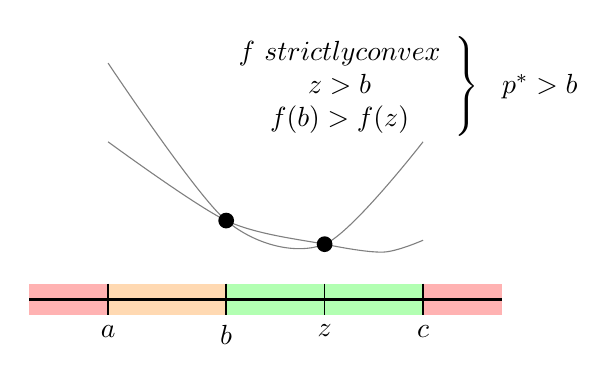
\begin{tikzpicture}
        \coordinate (c1) at (-0.5,1);
        \coordinate (c2) at (0.75,0.7);
        \fill[red,opacity=0.3] (-3,-.2) rectangle (-2,0.2);
        \fill[orange,opacity=0.3] (-2,-.2) rectangle (-0.5,0.2);
        \fill[green,opacity=0.3] (2,-.2) rectangle (-0.5,0.2);
        \fill[red,opacity=0.3] (2,-.2) rectangle (3,0.2);
        \draw[very thick] (-3,0) -- (3,0);
        \draw[thick] (-2,0.2) -- (-2,-0.2) node[below]{$a$};
        \draw[thick] (2,0.2) -- (2,-0.2) node[below]{$c$};
        \draw[] (0.75,0.2)  -- (0.75,-0.2) node[below]{$z$};
        \draw[thick] (-0.5,0.2) -- (-0.5,-0.2) node[below]{$b$};


        \draw[cyan,gray] plot [smooth] coordinates { (-2,2) (c1) (c2) (1.5,0.6) (2,0.75)};
        \draw[cyan,gray] plot [smooth] coordinates { (-2,3) (c1) (c2) (2,2)};

        \fill (c1) circle (0.1);
        \fill (c2) circle (0.1);

        \node[align=left] at (1.7,2.7) {$\left.\displaystyle\begin{array}{c}
            f~\text{strictly convex}\\
            z > b \\
            f(b) > f(z)
    \end{array}\right\}\implies~~p^* > b$};
    \end{tikzpicture}
\end{minipage}
\end{algorithm}

We begin by proving that \cref{algo:unimodal-search} does indeed output
a point within $\epsilon$ of
$p^*$.
Because $f$ is convex,
this algorithm satisfies an important invariant: 
    
\begin{iclaim} \label{claim:reduction-works}
    Both $b$ and $p^*$
    always lie in the interval $[a,c]$.
    \end{iclaim}
    \textit{Proof.~}
        We proceed by induction on $i$.
        At the beginning, it is obviously true that $b$ and $p^*$ lie in
        $[a,b] = [0,1]$, which contains the entire domain of $f$.
        Now, suppose inductively that $p^* \in [a,b]$ at some
        iteration of the algorithm $i$.
        \begin{itemize}[leftmargin=4em]
            \item [(case 1)] If $b-a \ge c-b$, then $z \in [a,b]$.
            \begin{itemize}[leftmargin=-1em]
                \item Suppose $f(z) < f(b)$. Then for
                all $y > b$, it must be the case that $f(y) > f(b)$ by convexity of $f$.
                (For if $f(y) < f(b)$, then segment between $(z, f(z))$ and $(y, f(y))$ would lie entirely below $(b, f(b))$, which contradicts convexity).
                Thus, we can rule out all such $y$ as possible minimizers of $f$, so
                we can restrict our attention to $[a, b]$, which contains $p^*$ (and $x$).

                \item On the other hand, if $f(z) > f(b)$, then it must be the case that no $y < z$ can be a minimizer of $f$ by convexity, with the same reasoning as above.
                (Namely, if $f(y) < f(z)$ then the segment between $(y,f(y))$ and $(b,f(b))$ lies below $(z,f(z))$, contradicting convexity).
                Thus the true minimizer $p^*$ lies in $[z,c]$, an interval which contains $b$.
            \end{itemize}
            \item [(case 2)] The other case is symmetric; we include it for completeness. Suppose $c-b > b-a$,
                and so $z = \frac{b+c}{2}$.
            \begin{itemize}[leftmargin=-1em]
                \item Suppose $f(z) < f(b)$. Then $f(y) > f(b)$ for  all $y < b$
                (because if $f(y) < f(b)$, then segment between $(y, f(y))$ and $(x, f(x))$ would lie  below $(b, f(b))$).
                So $p^*, z \in [b, c]$.

                \item On the other hand, if $f(z) > f(b)$, then $f(y) > f(z)$ for all $y > z$
                (because, if $f(y) < f(z)$ then the segment between $(y,f(y))$ and $(b,f(b))$ lies below $(z,f(z))$, contradicting convexity).
                So $p^*, b \in [a,z]$. \qedhere
            \end{itemize}
        \end{itemize}
        In every case, $p^*$ is still in what becomes
        the interval $[a,c]$ in the next iteration ($i+1$).
        So, by induction, $p^* \in [a,b]$ at every iteration of the algorithm,
        proving \cref{claim:reduction-works}.
        \qedsymbol

    We have shown that both $b$ and $p^*$ lie within $[a,c]$,
    and we know that, at termination, $|c-a| < \epsilon$.
    Therefore, the final value of $b$ (i.e., the output of the algorithm)
        must be within $\epsilon$ of $p^*$.




Next, we analyze the complexity of this algorithm, modulo the
    complexity of comparing the numbers $f(z)$ and $f(b)$, which
    we will later bound precisely.
    Each iteration reduces the size of the interval $[a,c]$
        by a factor of at least 3/4.
    This is because in each case we focus on the larger half of the interval,
        and ultimately discard either half or all of it---so
        we reduce the size of the interval by at least one quarter.
    It follows that, after $n$ iterations,
        the size of the interval is at most $(\nf34)^n$,
    and thus the total number of iterations is at most $\lceil\, \log(\nicefrac{1}{\epsilon}) / (\log \nicefrac43)\,\rceil$.
    Apart from the time needed to compare $f(b)$ and $f(z)$,
    it is easy to see that each iteration of the algorithm takes constant time.
    So overall, it requires
    $\log(\nf1\epsilon)$ space(enough to track the numbers $\{a,b,c\}$, plus a reference to the PDG $\dg M$), and time $O(\log \nf1\epsilon)$, (linear in the number of bits returned).
    This completes the proof of \cref{theorem:inf-via-inc-oracle} (a). 

    Although it is common to assume that numbers can be compared in $O(1)$ time, and this is an assumption well suited to modern computer architecture, it is arguably not appropriate in this context.
    How do we know a \texttt{float64} is has enough precision to do the comparison? 
The obvious approach to implementing the inconsistency calculation subroutine
    would be to repeatedly request more and more precise estimates of inconsistency,
    until one is larger than the other---but this procedure does not terminate if the two PDGs have the same inconsistency. 
    So, a priori, it's not even clear that the decision $f(b) > f(z)$
    is computable.
    It is not hard to show that it is in fact computable.
    Because $f$ is strictly convex,
    it must be the case that $f(b) > f(z)$, $f(z) > f(b)$, or
            $f(b) > f(\frac{b+z}{2})$.  
    In the last case, we can act as if $f(b) > f(z)$, and 
    the algorithm will be correct, because
    the argument supporting \cref{claim:reduction-works} still applies.
    Thus, by running the subroutine on all three questions until one of them
        returns true, and then aborting the other two calculations, we can see that
        the problem of interest is decidable.
    But how long does it take?
    We now provide a deeper analysis of the comparison between $f(z)$ and $f(b)$
    when the inconsistency calculation procedure can give us only finite approximations to the true value. 

    \textbf{Part (b): reduction to approximate inconsistency calculation.}
    Instead of assuming that we have direct access to the numbers $f(b)$ and $f(z)$ and
    can compare them in one step, we now adopt a weaker assumption, that we only have
    access to finite approximations to them.
    With this model of computation, it is not obvious that we can determine which of $f(b)$ and $f(z)$ is bigger---but fortunately, we do not need to.
    This is because, when $f(z)$ and $f(b)$ are close, $p^*$ lies between $z$ and $b$, and so both branches of the algorithm maintain the invariant $p^* \in [a,c]$.
    To simplify our analysis, we will default to keeping the ``left'' branch (with the smaller numbers), if the queried approximations to $f(z)$ and $f(b)$ are too close to determine whether one is larger than the other.

    More precisely, the test ``$f(z) \ll f(b)$'' is now shorthand
    for the following procedure:
    \begin{itemize}
        \item
        Run the inconsistency calculation procedure to obtain
        approximations to $f(z)$ and $f(b)$ that are correct to within
        \begin{equation}
            \epsilon' :=
            \frac{1}{16 \gamma}
                    \log^2 \Big(
                         1 +  8 \gamma (z-b)^2
                     \Big).
            \qquad\text{(This number comes from \cref{lem:togetherbound}.)}
            \label{eq:query-precision}
        \end{equation}
        Call these approximations $\tilde f(z)$ and $\tilde f(b)$.
        By definition, they satisfy $|f(z) - \tilde f(z)| \le \epsilon'$ and $|f(b) - \tilde f(b)| \le \epsilon'$.
        If $|\tilde f(z) - \tilde f(b)| > \epsilon'$ (so that we know for sure which of $f(z)$ and $f(b)$ is larger based on these approximations), then return
        TRUE If $\tilde f(z) < \tilde f(b)$, and FALSE otherwise.
        \item
        On the other hand, if $|\tilde f(z) - \tilde f(b)| \le \epsilon'$,
        return TRUE if $z < b$ and FALSE if $b > z$.
    \end{itemize}

    The remainder of the proof of correctness demonstrates that this level of precision is enough to never mistakenly eliminate the branch containing $p^*$.
    
    We begin by proving a series of three of additional invariants about the values $(a,b,z,c)$ in each iteration, which are required for our analysis.
    The first property is
    that $b$ and $z$ are not too close to the boundary or each other.

    \begin{iclaim} \label{claim:b-z-eps-sep}
        At the beginning of each iteration,
        \[
        b \in [\frac\epsilon2, 1-\frac\epsilon2],\qquad
        z \in [\frac\epsilon4, 1-\frac\epsilon4],\quad\text{and}\quad
        |b-z| \ge \frac{\epsilon}{4}.\qedhere
        \]
    \end{iclaim}
    We prove this by contradiction.
    Initially, $b = \frac12$
    so it's neither the case that $b < \frac\epsilon2$ nor that $b > 1-\frac\epsilon2$
    for any $\epsilon < 1$. (The procedure terminates immediately
        if  $\epsilon \ge 1$.)
    In search of a contradiction,
        suppose that either $b < \frac\epsilon2$ or $b > 1 - \frac\epsilon2$ later on.
    Specifically, suppose it first occurs in the $(t+1)^{\text{st}}$ iteration,
        and let $(a_{t+1},b_{t+1},c_{t+1})$ to refer to the values of
        $(a,b,c)$ in that iteration.
    Let $(a_t, b_t, z_t, c_t)$ denote the values of the variables
        in the previous iteration.
    We know that $b_{t+1} \notin [\frac\epsilon2, 1-\frac\epsilon2]$
        and $b_t \in [\frac\epsilon2, 1-\frac\epsilon2]$.
    In particular, $b_{t} \ne b_{t+1}$, which means the procedure
        cannot have taken the second or fourth branches in the $t^{\text{th}}$ iteration.
    There are two remaining cases, corresponding to the first
        and third branches.
    \begin{itemize}
    \item \textbf{(branch 1)~~} In this case, $b_t-a_t \ge c_t - b_t$ and $z_t = {(a_t+b_t)}/2$.  Furthermore, as a result of the assignment in this branch, we have $c_{t+1} = b_t$ and
            $b_{t+1} =  z_t  = {(a_t+b_t)}/2$.
    \begin{itemize}
        \item
        If $b_{t+1} < \frac\epsilon2$, this means $a_t + b_t < \epsilon$.
        As $a_t \ge 0$, this implies $b_{t} = c_{t+1} < \epsilon$.
        But then $|c_{t+1} - a_{t+1}| \le c_{t+1} < \epsilon$, so the algorithm must
        have already terminated! This is a contradiction.
        \item
        If $b_{t+1} > 1-\frac\epsilon2$, then
        $1- \frac\epsilon2 < b_{t+1} = z_t = (a_t+b_t)/2 < b_t$,
        contradicting our assumption that $b_t \le 1-\frac\epsilon2$.
    \end{itemize}


     \item \textbf{(branch 3)~~} In this case, $c_t-b_t > b_t - a_t$ and $z_t = ({b_t+c_t})/2$.
     The assignment at the end of this branch ensures that
        $a_{t+1}=b_t$ and $b_{t+1}=z_t$.
    \begin{itemize}
    \item
     If $b_{t+1} < \frac\epsilon2$, then
         $b_t = a_{t+1} < b_{t+1} < \frac\epsilon2$.
         which is a contradiction.
    \item
        If $b_{t+1} = ({b_t+c_t})/2 > 1-\frac\epsilon2$, then,
        since $c_t \le 1$, we know $b_t + 1 > 2 - \epsilon$, so $b_t = a_{t+1} > 1-\epsilon$.
        But now $|c_{t+1} - a_{t+1}| \le 1 - a_{t+1} < 1- (1-\epsilon) = \epsilon$.
        So the algorithm must have already terminated.
    \end{itemize}
    \end{itemize}
    Thus, it cannot be the case that $b < \frac\epsilon2$ or $b > 1-\frac\epsilon2$ in any iteration of the algorithm. The fact that $z \in [\frac\epsilon4,1-\frac\epsilon4]$ follows immediately from the definition of $z$ in either branch.
    Finally, $|z-b| = \frac12 \max\{c-b, b-a\} \ge \frac12(\frac{c-a}{2}) > \frac\epsilon4$.
    This completes the proof of \cref{claim:b-z-eps-sep}. \qedsymbol


    \begin{iclaim}\label{claim:b-middlethird}
        It is always the case that $b \in [ \frac{2a + c}{3}, \frac{a + 2c}{3}]$.
    \end{iclaim}
    We prove this by induction. It is clearly true at initialization;
    suppose it is also true at time $t$, i.e., $\frac{2 a_t + c_t}{3} \le b_t \le \frac{a_t + 2 c_t}{3}$.
    We now show the same is true at time $t+1$ in each of the four cases of the algorithm.
    \begin{itemize}
        \item \textbf{(branch 1)~~}
            At the end, we assign
                $a_{t+1} = a_t$,
                $b_{t+1} = z = \frac{a_t + b_t}{2}$, and
                $c_{t+1} = b_t$.
            So,
            \begin{align*}
                \frac{2 a_{t+1} + c_{t+1}}{3}
                = \frac{2 a_t + b_t}{3} <
                ~~\underbrace{~~\frac{a_t+b_t}{2}~~}_{\textstyle = b_{t+1}}~~
                < \frac{a_t + 2 b_{t}}{3} =
                \frac{a_{t+1} + 2 c_{t+1}}{3}.
            \end{align*}

        \item \textbf{(branch 2)~~}
        In this case, we must make use of the fact that, in the first
        two branches  $b-a \ge c-b$, meaning $a_t + c_t \le 2b_t$.
        As in the first branch, we have $z = \frac{a_t + b_t}{2}$.
        This time, however,
            $a_{t+1} = z = \frac{a_t + b_t}{2}$,
            $b_{t+1} = b_t$, and
            $c_{t+1} = c_t$.
        Thus, we find
        \begin{align*}
            \frac{2 a_{t+1} + c_{t+1}}{3}
            = \frac{a_t + b_t + c_t}{3}
            &\le \frac{(2b_t) + b_t}{3}
            = b_t \\
            &= b_{t+1}
            \le \frac{a_t + 2 c_{t}}{3}
            < \frac{\frac{a_t + b_t}2 + 2 c_{t}}{3}
            = \frac{a_{t+1} + 2 c_{t+1}}{3} .
        \end{align*}

        \item \textbf{(branch 3)~~} Symmetric with branch 1.
        Concretely,
            $a_{t+1} = b_t$,
            $b_{t+1} = z = \frac{b_t + c_t}2$, and
            $c_{t+1} = c_t$. Thus,
        \begin{align*}
            \frac{2 a_{t+1} + c_{t+1}}{3}
            = \frac{2 b_t + c_t}{3} <
            ~~\underbrace{~~\frac{b_t+c_t}{2}~~}_{\textstyle = b_{t+1}}~~
            < \frac{b_t + 2 c_{t}}{3} =
            \frac{a_{t+1} + 2 c_{t+1}}{3}.
        \end{align*}

        \item  \textbf{(branch 4)~~} Symmetric with branch 2.
        Concretely,
            $a_{t+1} = a_t$,
            $b_{t+1} = b_t$,
            $c_{t+1} = z = \frac{b_t+ c_t}2$,
        and we know $2 b_t < a_t + c_t$.
        Thus,
        \begin{align*}
            \frac{2 a_{t+1} + c_{t+1}}{3}
            = \frac{2 a_{t} + \frac{c_{t} + b_t}2}{3}
            &< \frac{2 a_t + c_t}{3}
            \le b_t \\
            &= b_{t+1}
            = \frac{2 b_t + b_t}{3}
            < \frac{(a_t + c_t) + b_t}3
            = \frac{a_{t+1} + 2 c_{t+1}}3
            .
        \end{align*}
    \end{itemize}

    The final result we need is a bound for \cref{lem:togetherbound}. 
    
    \begin{iclaim}\label{claim:logbz-bound}
        $| \log \frac{z}{b} \frac{1-b}{1-z} | \le \log 4
            ~~(< \sqrt{2})$.
    \end{iclaim}
    \textit{Proof.}
    Let $\bar a := 1-a$, $\bar b := 1-b$, and $\bar c := 1-c$. 
    \Cref{claim:b-middlethird} tells us that
    $ b \ge \frac{2a + c}3 \ge \frac c3$, and also that $b \le \frac{a+2c}3$,
    which gives us a symmetric fact:
    $
        \bar b = 1-b \ge \frac33 - \frac a3 - \frac{2c}3 = \frac{\bar a + 2 \bar c}{3} \ge \frac{\bar a}3.
    $
    Consider two cases, corresponding to the two definitions of $z$. 
    Either $z = (a+b)/2$ or $z = (b+c)/2$.
    
    \begin{minipage}{0.49\linewidth}
        \textbf{Case 1.} $\frac{a+b}2 = z < b$. Thus,
        \begin{align*}
            \Big| \log & \frac zb  \frac{1-b}{1-z} \Big| 
            = \log \frac bz \frac{1-z}{1-b} \\
            &= \log \frac {2b}{a+b} \frac{1-\frac{a+b}2}{1-b} \\
            &= \log \frac {b}{a+b} \frac{2 - a - b}{1-b} \\
            &= \log \frac {b}{a+b} + \log \frac{\bar a + \bar b}{\bar b} \\
            &\le \log \frac{\bar a + \bar b}{\bar b}
                \qquad \Big[\parbox{2.6cm}{\centering\singlespacing as first term\\ is negative}\Big] \\
            &= \log\Big(1 + \nicefrac{\bar a}{\bar b}\Big) \\
            &\le \log \Big(1 + \frac{\bar a}{(\bar a / 3)} \Big)
            = \log 4.
        \end{align*}
    \end{minipage}
    \begin{minipage}{0.49\linewidth}
        \textbf{Case 2.}
        $\frac{b+c}2 = z > b$. Thus,
        \begin{align*}
            \Big| \log & \frac zb \frac{1-b}{1-z} \Big| 
            = \log \frac zb \frac{1-b}{1-z} \\
            &= \log \frac {b+c}{2b} \frac{1-b}{1-\frac{b+c}2} \\
            &= \log \frac {b+c}{b} \frac{1-b}{2 - b - c} \\
            &= \log \frac {b+c}{b} + \log \frac{\bar b}{\bar b + \bar c} \\
            &\le \log \frac{b + c}{b}
                \quad~~ \Big[\parbox{2.85cm}{\centering\singlespacing as second term\\ is negative}\Big] \\
            &= \log\Big(1 + \nicefrac{c}{b}\Big) \\
            &\le \log \Big(1 + \frac{c}{(c / 3)} \Big)
            = \log 4.
        \end{align*}
    \end{minipage}
    \qedsymbol


    We are now in a position to prove that we never mistakenly eliminate $p^*$
    when comparing truncated representations.
    Without loss of generality, suppose that $z > b$, as the two cases are symmetric.
    Since we choose the left branch in the event of a tie, we have made a mistake
        if we instead needed to have chosen the right branch: $p^* > z$.
    In search of a contradiction, suppose that indeed
        this is the case.
    Under these conditions (i.e., $b < z < p^*$), and in light of \cref{claim:logbz-bound},
    we can apply \cref{lem:togetherbound} with $k = \sqrt{2} > \ln 4$, which tells us that
    \begin{align*}
        f(b) - f(z)
        &>
        \frac{1}{16 \gamma}
        \log^2 \Big(
            1 +  8 \gamma (z-b)^2
        \Big).
    \end{align*}
    The definition of $\epsilon'$ in \eqref{eq:query-precision} is constructed
    precisely to make sure that this is never true.
Therefore, the algorithm cannot choose the wrong branch.





    \textbf{Complexity Analysis.}
    We now provide a more careful analysis of the runtime of the algorithm.
    We already have a bound on the number of iterations required;
    what is missing is a bound on how long it takes to compute $\ll$, i.e., to compare the approximations $\tilde f(z)$ and $\tilde f(b)$.
    Assuming these numbers are in binary format, $\tilde f(z)$ is of the form $A.B$, and $\tilde f(b)$ is of the form $A'.B'$, where $\{A, A', B, B'\}$ are binary sequences.

    Without loss of generality, assume that $|A| \le |A'|$. (Otherwise, swap their labels.)  The complexity of comparing the two numbers $\tilde f(z)$ and $\tilde f(b)$ does not depend on $|A'|$, the longer of the two sequences to the left of the radix point.
    This is because once we see the radix point in one number but not the other, we can immediately conclude the former is smaller.
    In the first iteration, $|A|$ is at most
    \begin{align*}
        |A| &\le \max \left\{ 0,~ \log_2 \aar[\Big]{\dg M ~+~ \Pr(Y{=}y){=}\frac12}_{\!\gamma} \right\} \\
        &\le
            \max \left\{ 0,~ \log \Big( \aar{\dg M}_\gamma
        +
            \kldiv{p^*}{.5}
        \Big)
         \right\}\\
         &\le \log_2\Big( \max \{ 0, \aar{\dg M}_\gamma \} + 1 \Big)
         \qquad \big[~\text{since }\kldiv{p}{.5} \le 1~\big]
         \\&\in O( \log \aar{\dg M}_\gamma )
         .
    \end{align*}
    Furthermore, $|A|$ cannot increase as the algorithm progresses, because whichever of $\{z, b\}$ leads to a smaller value of $f$ becomes the new value of $b$ in the following iteration.

    Next, we derive an upper bound on the number of bits of $B$ and $B'$ that we must compare.
    Taking the (base-2) logarithm of \eqref{eq:query-precision}, we find that
    we need to examine at most
    \begin{align*}
        |B| ~&\le~ 4 + \log_2 (\gamma)
            - 2 \log_2 \log \left(1 +  8 \gamma (z-b)^2 \right)
        \\&\le~
            4 + \log_2 ({\gamma})
            - 2 \log_2 \log \left(1 +  \frac1{2} \gamma \epsilon^2\right)
            & \Big[~\text{since $(z-b) \ge \frac\epsilon4$}~\Big]
    \end{align*}
    bits to the right of the radix point in order to eliminate the possibility that $f(b) < f(z)$. 
    This expression is still not very friendly; we now loosen it even further to provide a bound of a simpler, more recognizable form.
    When $x \ge 0$, we know that $\log(1 + x) \ge  1- \frac{1}{1+x} = \frac{x}{x+1}$;
    it follows that $-\log_2 \log(1+x) \le -\log_2(\frac{x}{x+1})
         = \log_2( 1+ \frac1x)$.
    Thus,
    \begin{align*}
        |B| + |A| \ &\le 4 + \log_2(\gamma) + 2 \log_2
        \left(1 + \frac{2}{\gamma\epsilon^2 }\right)
        + \log_2\Big( \aar{\dg M}_\gamma + 1 \Big)\\
        &\in O \left(\log\frac1\epsilon + |\log {\gamma}\, | + \log\aar{\dg M}_\gamma \right).
    \end{align*}

    Recall that the process takes at most $O(\log \frac1\epsilon)$ iterations---but in the process, produces the same number of bits of output, since $\log(\nf1\epsilon)$ is the number of bits need to encode the final approximation to $p^*$.
    So, accounting for the time needed to compare $f(z)$ and $f(b)$,
        the algorithm runs in time
    \begin{align*}
        O \left(
        \log \frac1\epsilon
        ~\cdot~
        \Big(\log \frac1{\gamma}
        + \log \frac1\epsilon
        + \log \aar{\dg M}_\gamma
        \Big)
        \right).
    \end{align*}
    
    At this point, we have shown reduced unconditional inference to inconsistency calculation. To extend the reduction to conditional queries, we can apply \cref{lem:logeps-conditioner} with 
    $k=2$, 
    $K_0 = 0$, 
    $K_1 = \log \frac1\gamma + \log(1 + \aar{\dg M}_\gamma)$, 
    $K_2 = 1$, and $\Phi = 1$, 
    to get an algorithm that runs in
    \begin{align*}
        O \left(
        \Big(\log \frac1{\gamma}
        + \log \aar{\dg M}_\gamma
        \Big)
        \cdot
        \log \frac1{\epsilon\, \mu^*\mskip-2mu(X{=}x)}
        +
        \log^2 \frac1{\epsilon\, \mu^*\mskip-2mu(X{=}x)}
        \right)
        ~~\text{time}.
    \end{align*}
    It uses $O(\log \log \frac1{\mu^*(X{=}x)} \cdot \log \frac1\epsilon)$ 
        calls to the inconsistency calculation procedure.     
    





    Finally, we remark that
    typically we are interested in doing inference up to floating point 
    precision.
    In this case, by selecting
$\epsilon \le 10^{-78}$, the procedure above
runs in constant time, making at most 1555 
    inconsistency procedure calls before outputting
     the 64-bit float that is closest to $p^*$.

    \textbf{The other direction: reducing inconsistency calculation to inference.}
    This reduction is much simpler, shares more techniques with the primary
    thrust of the paper. First find a tree
    decomposition $(\C, \mathcal T)$ of the PDG's structure,
    and then query the marginals of each clique.  Because of the
    work we've already done, we know this information is enough
    information to simply evaluate the scoring function,
    including the joint entropy, by \eqref{eq:cluster-ent-decomp}.
\end{lproof}

% \end{subappendices}
